\documentclass[11pt,a4paper]{article}
\usepackage[margin=3cm]{geometry}
\usepackage[utf8]{inputenc}
\usepackage{listings}
\usepackage{courier}
\usepackage{amsmath}
\usepackage{amsfonts}
\usepackage{amssymb}
\usepackage{makeidx}
\usepackage{graphicx}
\usepackage{hyperref}
\usepackage{indentfirst}
\usepackage{xcolor}
\usepackage{epsfig}
% -- code style text box
\usepackage{titling}
\newcommand{\subtitle}[1]{%
	\posttitle{%
		\par\end{center}
	\begin{center}\large#1\end{center}
	\vskip0.5em}%
    % http://tex.stackexchange.com/questions/50182/subtitle-with-the-maketitle-page
}
% -- fonts
\usepackage{fontspec}
\setmainfont{RomanSerif}
\setsansfont{Overlock}
\setmonofont{Inconsolata}
% -- xmark
\newcommand{\xmark}{\textcolor{green!50!black}{x}}
% -- table font size -- http://tex.stackexchange.com/questions/27097/changing-the-font-size-in-a-table
\usepackage{floatrow}
\DeclareFloatFont{large}{\large} % "scriptsize" is defined by floatrow, "tiny" not
\floatsetup[table]{font=large}
% -- author, title
\author{}
\title{Superdeblending Manual}
\subtitle{(GOODS-North)}
\begin{document}
\maketitle
\tableofcontents
\clearpage
\setlength{\baselineskip}{16pt}
\setlength{\parskip}{5pt}

\lstset{
	numbers=left,
	stepnumber=1,
	numbersep=10pt,
	numberstyle=\footnotesize,
	basicstyle=\footnotesize\ttfamily,
	keywordstyle=\color{blue!70},
	commentstyle=\color{red!50!green!50!blue!50},
	frame=shadowbox,
	rulesepcolor=\color{red!20!green!20!blue!20},
	escapeinside=``,
	xleftmargin=2em,
	xrightmargin=0em,
	aboveskip=1em,
	tabsize=4,
	showspaces=false,
	showstringspaces=false
}

%*************************************************************************************
\section{Abstract}

This is the manual for the 24+radio catalog. We use the whole IRAC catalog as the prior source list for PSF fitting photometry, then use Monte-Carlo simulation to validate and correct measurements. The output is a catalog contains IRAC, Ks, 24 and radio band flux and uncertainties. Additional, we measure 16um based on this catalog, and append 16um flux and uncertainty to our final 24+radio catalog. 

\vspace{5cm}
Hints: black text are our method and procedures, \textcolor{blue}{blue text are notes}, and \textcolor{red}{red text are unsolved issues.}

%*************************************************************************************

\clearpage

%*************************************************************************************
\section{Dashboard}

\begin{figure}[H]
	\caption{{\Large Flow chart diagram}\newline Processing: Initial Catalog $\to$ SED $\to$ predict $\to$ subtract $\to$ galfit $\to$ residual $\to$ simulation $\to$ statistical corrections $\to$ final catalog and SED.}
	\centering
	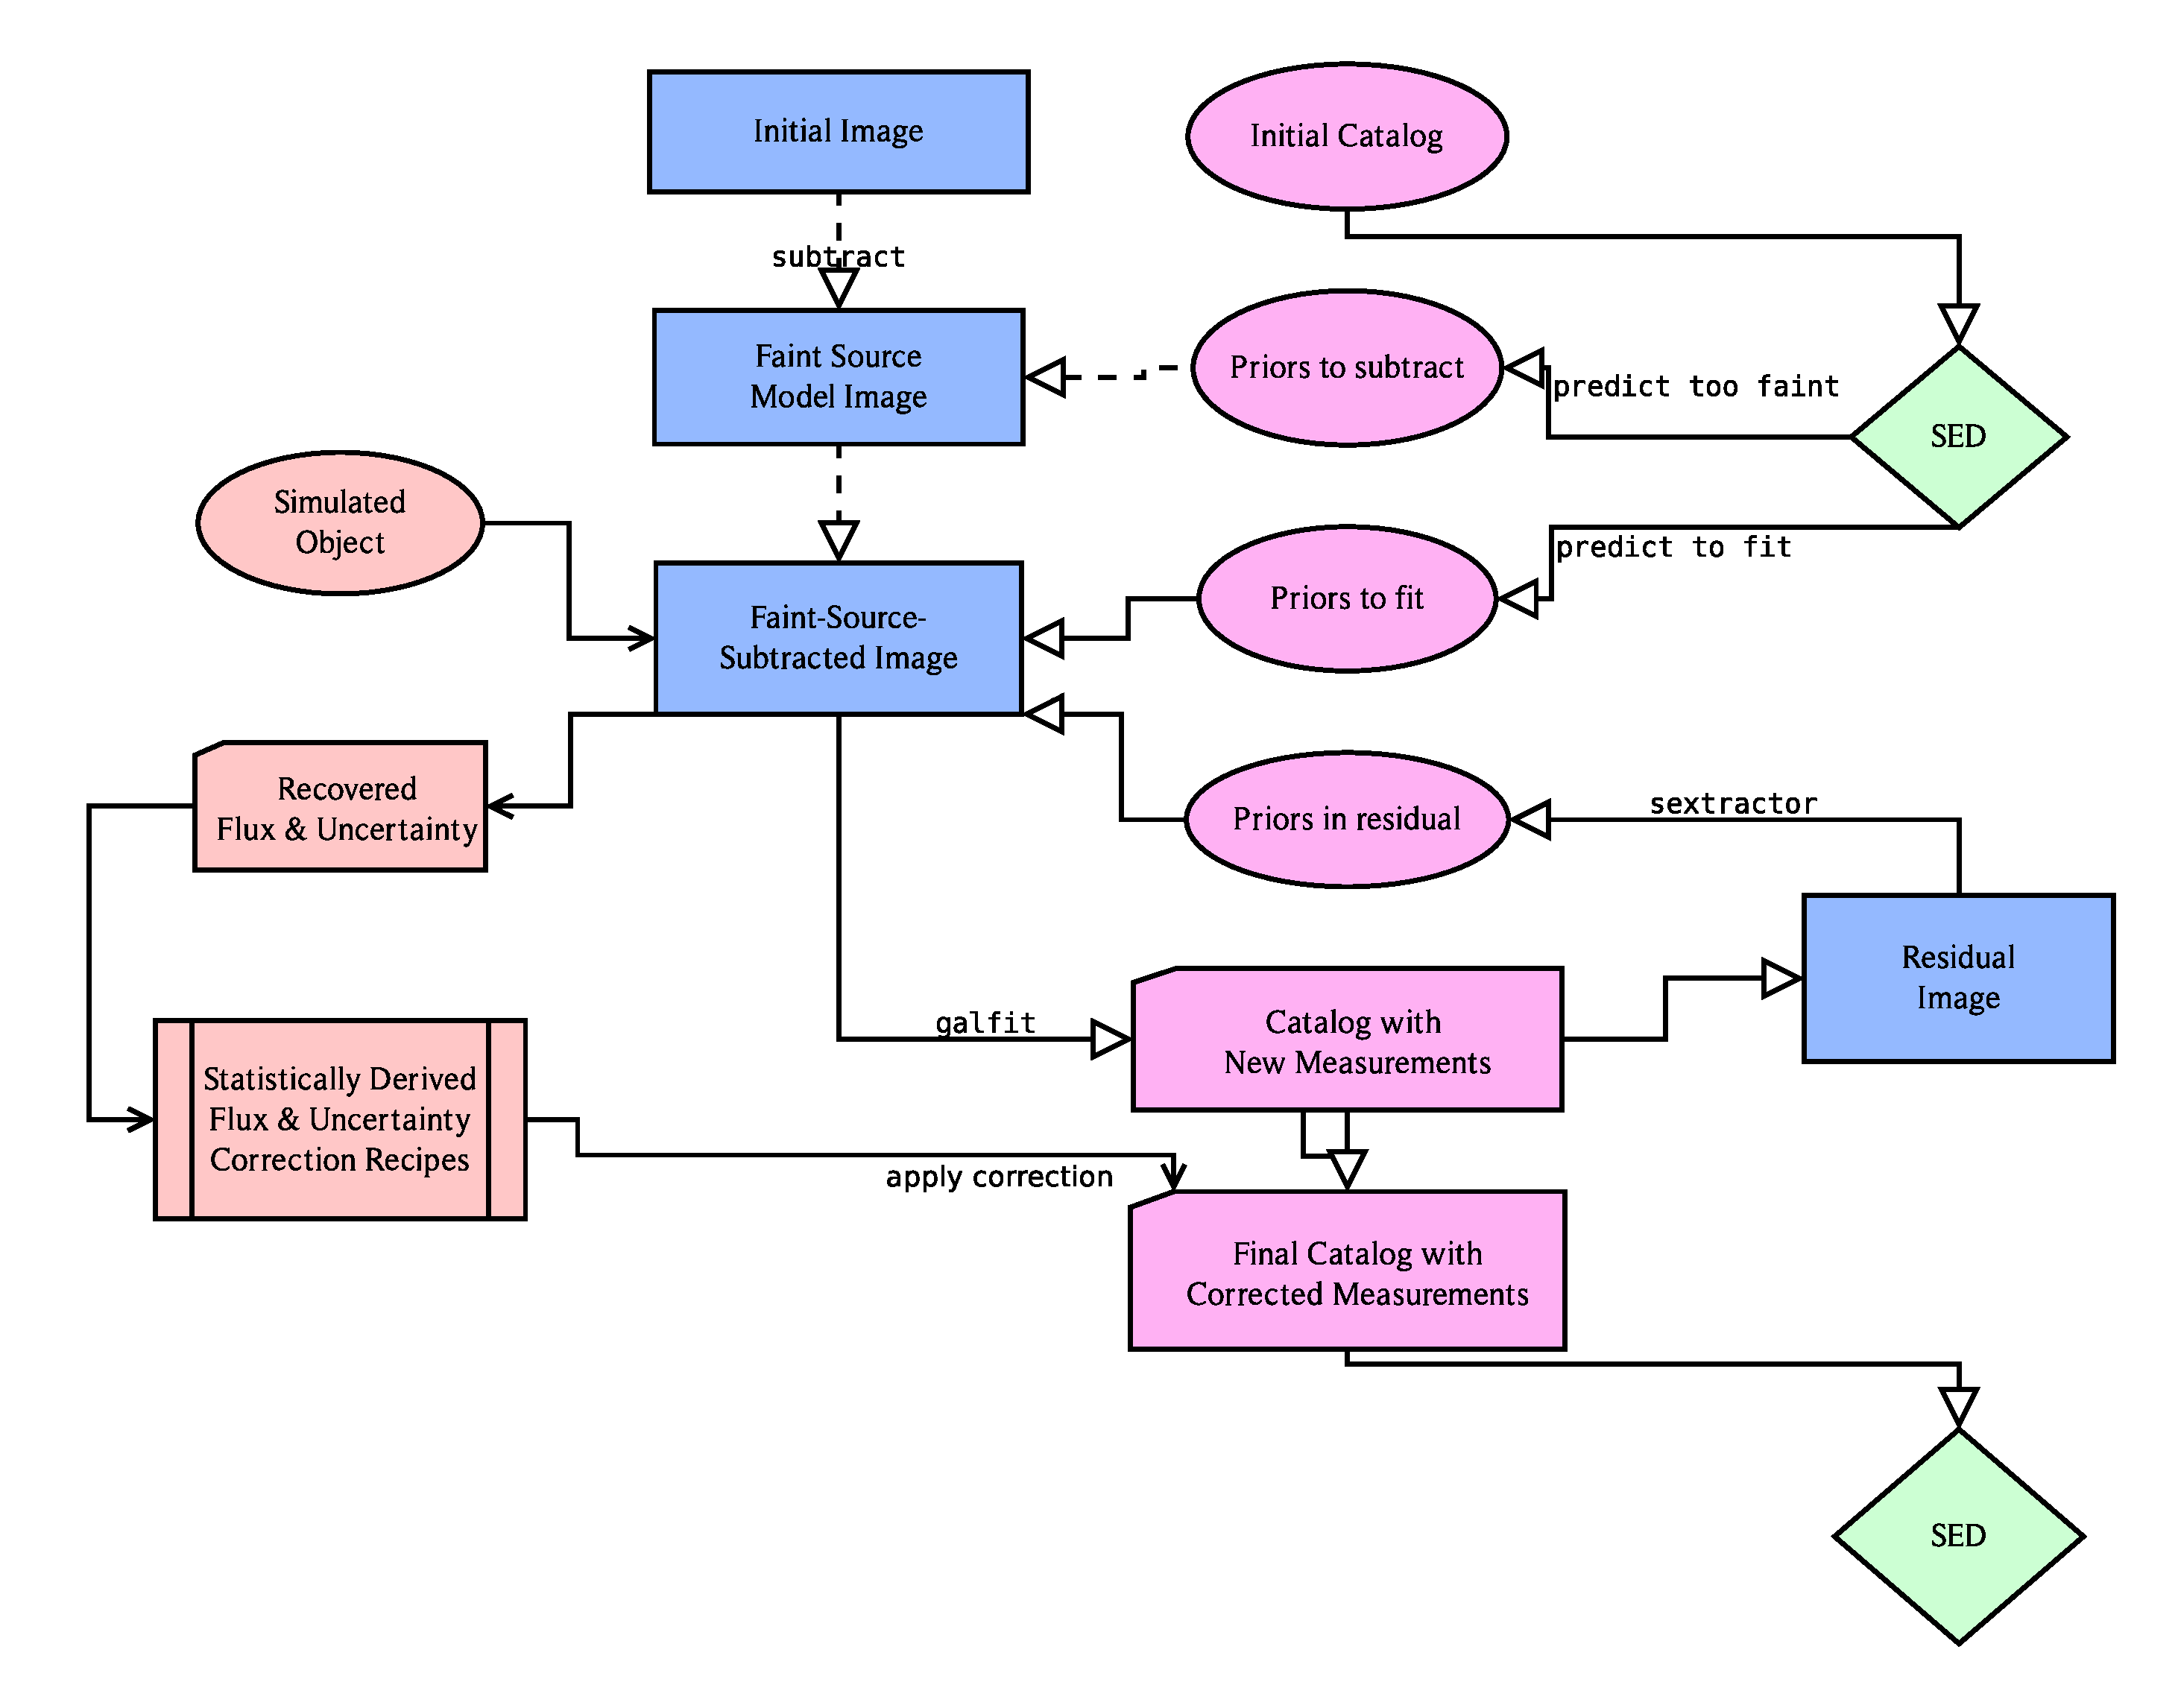
\includegraphics[width=0.92\textwidth]{FlowChartDiagram}
\end{figure}


\begin{table}[h]
	%\centering % -- use the floatrow package (this also saves typing \centering in every table):
	\caption{\Large Status of Processing}
	\begin{tabular}{ccccccccc}
		\hline
		\hline
		Band & SED & Predict & Subtract & Galfit & Residual & Galsim & Correct & Final \\
		& 1 & 2 & 3 & 4 & 5 & 6 & 7 & 8 \\
		\hline
		100 & [\ref{Band100_Galsed}] & [\ref{Band100_Galpre}] & [\ref{Band100_Galsub}] & [\ref{Band100_Galfit}] & [\ref{Band100_Galres}] & [\ref{Band100_Galsim}] & [\ref{Band100_dfcorr}] & [\xmark] \\
		160 & [\ref{Band160_Galsed}] & [\ref{Band160_Galpre}] & [\ref{Band160_Galsub}] & [\ref{Band160_Galfit}] & [\ref{Band160_Galres}] & [\ref{Band160_Galsim}] & [\ref{Band160_dfcorr}] & [\xmark] \\
		250 & [\ref{Band250_Galsed}] & [\ref{Band250_Galpre}] & [\ref{Band250_Galsub}] & [\ref{Band250_Galfit}] & [\ref{Band250_Galres}] & [\ref{Band250_Galsim}] & [\ref{Band250_dfcorr}] & [\xmark] \\
		350 & [\ref{Band350_Galsed}] & [\ref{Band350_Galpre}] & [\ref{Band350_Galsub}] & [\ref{Band350_Galfit}] & [\ref{Band350_Galres}] & [\ref{Band350_Galsim}] & [\ref{Band350_dfcorr}] & [\xmark] \\
		500 & [\ref{Band500_Galsed}] & [\ref{Band500_Galpre}] & [\ref{Band500_Galsub}] & [\ref{Band500_Galfit}] & [\ref{Band500_Galres}] & [\ref{Band500_Galsim}] & [\ref{Band500_dfcorr}] & [\xmark] \\
		1160 & [\ref{Band1160_Galsed}] & [\ref{Band1160_Galpre}] & [\ref{Band1160_Galsub}] & [\ref{Band1160_Galfit}] & [\ref{Band1160_Galres}] & [\ref{Band1160_Galsim}] & [\ref{Band1160_dfcorr}] & [\xmark] \\
		\hline
	\end{tabular}
\end{table}

%*************************************************************************************

\clearpage

%*************************************************************************************
\section{Band 100}

%*************************************************************************************
\subsection{SED fitting before band 100}
\label{Band100_Galsed}

The SED fitting at this step includes these bands: 

\indent\hspace{15pt}$\bullet$ $K_s$
\\
\indent\hspace{15pt}$\bullet$ IRAC 3.6, 4.5, 5.8, 8.0
\\
\indent\hspace{15pt}$\bullet$ IRS PUI 16, MIPS 24
\\
\indent\hspace{15pt}$\bullet$ VLA 1.4 GHz (hereafter radio) 
\\

The SED fitting uses the following 3 parameters for better fitting of the SEDs: 

\indent\hspace{15pt}$\bullet$ 
Type\_AGN: radio loud AGN, 
$(f_{radio}-f_{SED}) > 3\times\sqrt{\sigma_{f_{radio}}^2+\sigma_{f_{SED}}^2}$
\\
\indent\hspace{15pt}$\bullet$ 
Type\_SED: pure starburst, 
$SFR_{SED} > 6\times{SFR}_{MS}$
\\
\indent\hspace{15pt}$\bullet$ 
Type\_FIR: high FIR S/N ratio, 
$\sqrt{SNR_{100}^2+\cdots+SNR_{1160}^2}>10$
\\

But at this step, we do not have any prior information about these Type\_ parameters. 
Therefore, we run a trial SED fitting without any Type\_ parameter, and use the output to do the Type\_AGN and Type\_SED classifications: 

\indent\hspace{15pt}$\bullet$ 
Type\_AGN: 85 out of 3306 sources are classified as radio loud AGN, for which we will not fit their radio data points. 
\\
\indent\hspace{15pt}$\bullet$ 
Type\_SED: 46 out of 3306 sources are classified as pure starburst (hereafter SB), for which we will use only SB type SED templates. 1011 out of 3306 sources are classified as pure main-sequence (hereafter MS), for which we will use only MS type SED templates. 
\\

Applying these Type\_ parameters, we run the SED fitting again, and use the results for the next step SED prediction. Additionally, we update the Type\_ parameters, but do not repeat a third fitting for now. 

\indent\hspace{15pt}$\bullet$ 
Type\_AGN: 205 radio AGNs, 3306 in total. 
\\
\indent\hspace{15pt}$\bullet$ 
Type\_SED: 41 pure SB, 891 pure MS, 3306 in total. 
\\
\indent\hspace{15pt}$\circ$ 
\textcolor{blue}{Comparing to the trial step SED fitting: applying Type\_AGN leads to lower SED best fitting SFR and S/N ratio for some radio AGNs, therefore their Type\_SED changed from pure MS to unclassified.}
\\
\indent\hspace{15pt}$\circ$ 
\textcolor{blue}{Code update: 2015-12: introduced a new parameter Type\_FIR, but this parameter is not determined from SED fitting results but the galfit photometry results. This parameter will be used since the SED fitting before band 160, but not current step before band 100.}
\\


\subsection{SED prediction for band 100}
\label{Band100_Galpre}

We use SED best fitting flux and uncertainty at band 100 as the predicted values to flag faint sources. We set a $(f+2\sigma_{f})$ cut $f_{cut}$, so that brighter or larger uncertainty sources will be kept while fainter and better constrained sources will be flagged and subtracted. A Type\_FIT parameter is determined for each source from the SED best fitting results:

\indent\hspace{15pt}$\bullet$ 
Type\_FIT: fit at current band, $(f_{SED}+2\sigma_{f_{SED}})/crowdiness > f_{cut}$
\\
\indent\hspace{15pt}$\circ$ 
\textcolor{blue}{DONE: 2015-12: I'm thinking about a crowdiness-dependent way to flag sources, so that if a source is relatively isolated, we can use a lower $f_{cut}$ which tends to keep it for fitting, while a source is in a relatively blended environment, we can use a higher $f_{cut}$ so that it tends to be flagged out. The inequation thus becomes $(f_{SED}+2\sigma_{f_{SED}})/crowdiness \ge f_{cut}$.}
\\
\indent\hspace{15pt}$\circ$ 
\textcolor{blue}{NOTE: 2015-12: The ''crowdiness'' property of a prior source is the sum of the Gaussian-type weights of all surrounding sources including the source itself: 
\\
$crowdiness_{i} = \sum_{j=1}^{N} \, e^{-4\ln{2}\cdot\left((\mathrm{RA}_{j}-\mathrm{RA}_{i})^2+(\mathrm{Dec}_{j}-\mathrm{Dec}_{i})^2\right)/\left(\mathrm{FWHM}\right)^2}$. }
\\
\indent\hspace{15pt}$\circ$ 
\textcolor{blue}{DONE: 2015-12: I have computed the ''crowdiness'' values using this equation, and with proper FWHM values as recorded in ''goFine.sm'' and ''astroPhot.sm''. Note that the computations before were normalized to arbitary value and were not using proper FWHM at each band. }
\\

With different $f_{cut}$, the number of faint sources that are flagged out changes, and the number of sources kept for fitting also changes as a function of $f_{cut}$. Dividing the number of sources by the PSF beam area: $A_\mathrm{PSF}={\pi}/({4\ln{2})}\cdot\mathrm{FWHM}^2$, the density of sources for fitting ($\rho_{fit}$) can be derived. We decide the best $f_{cut}$ value by ensuring that  $\rho_{fit}$ is not larger than 1 source per beam, so that the photometry performance can be improved. 

%% 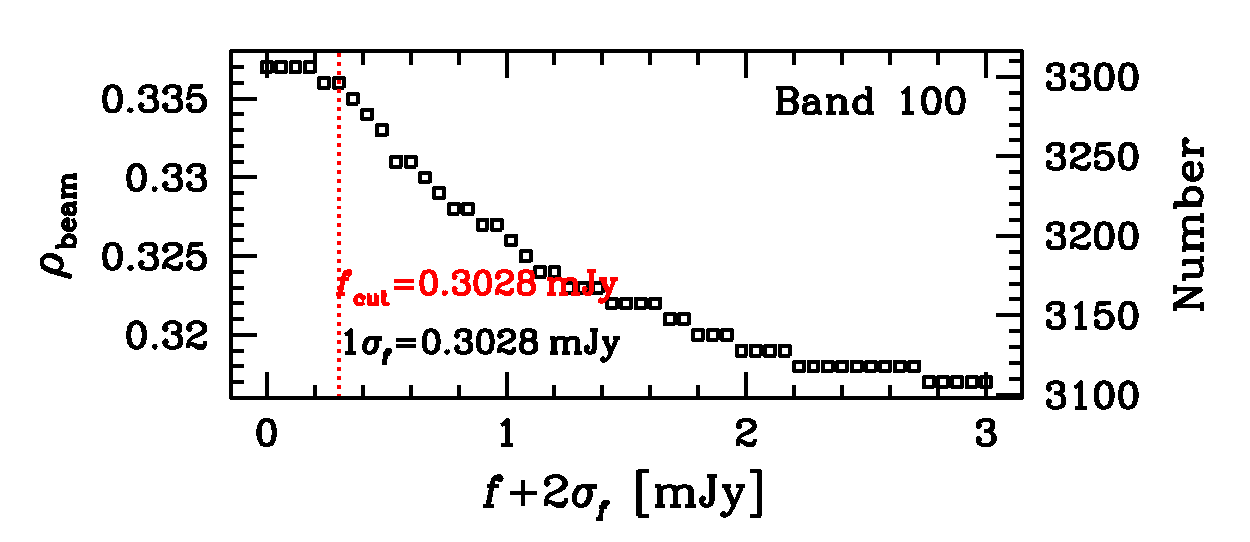
\includegraphics[width=0.45\textwidth]{plot_cutting_flux_100}
%% 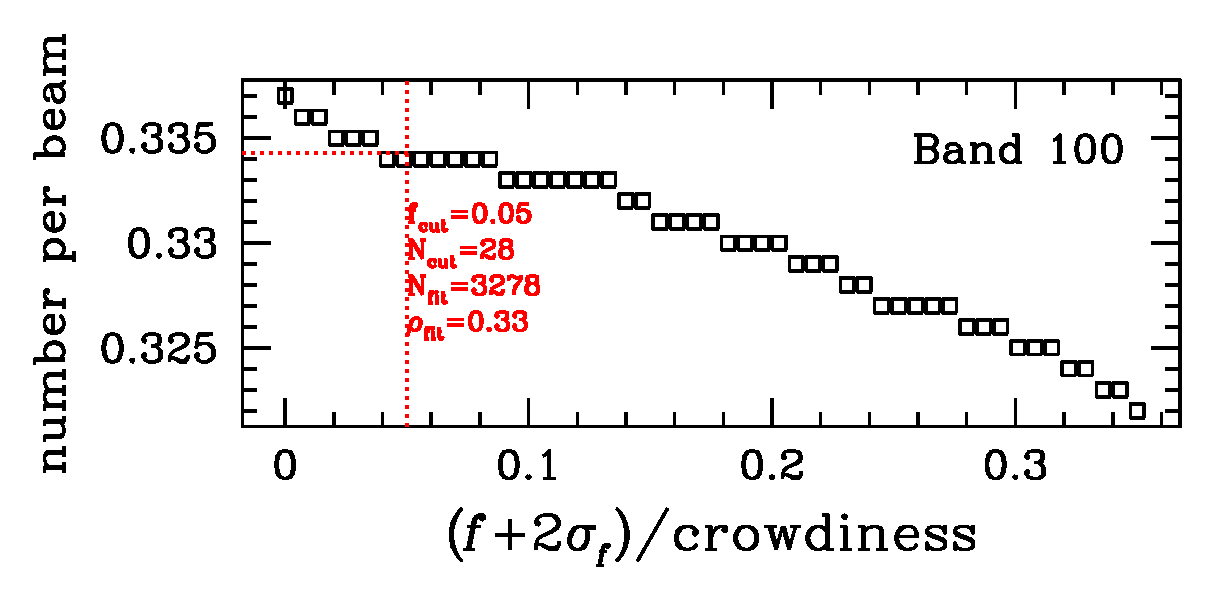
\includegraphics[width=0.45\textwidth]{plot_cutting_flux_100_with_crow}

\begin{figure}[H]
	\caption{Number of sources kept for fitting per PSF beam area ($\rho_{fit}$) as a function of different $f_{cut}$ at band 100. $\rho_{fit}$ is small at band 100, therefore even without flagging out any sources, the photometry performance can still be good. But we still decide to set a very low $f_{cut}$ to flag out a few sources that are predicted to be too faint or in too crowd environment.}
	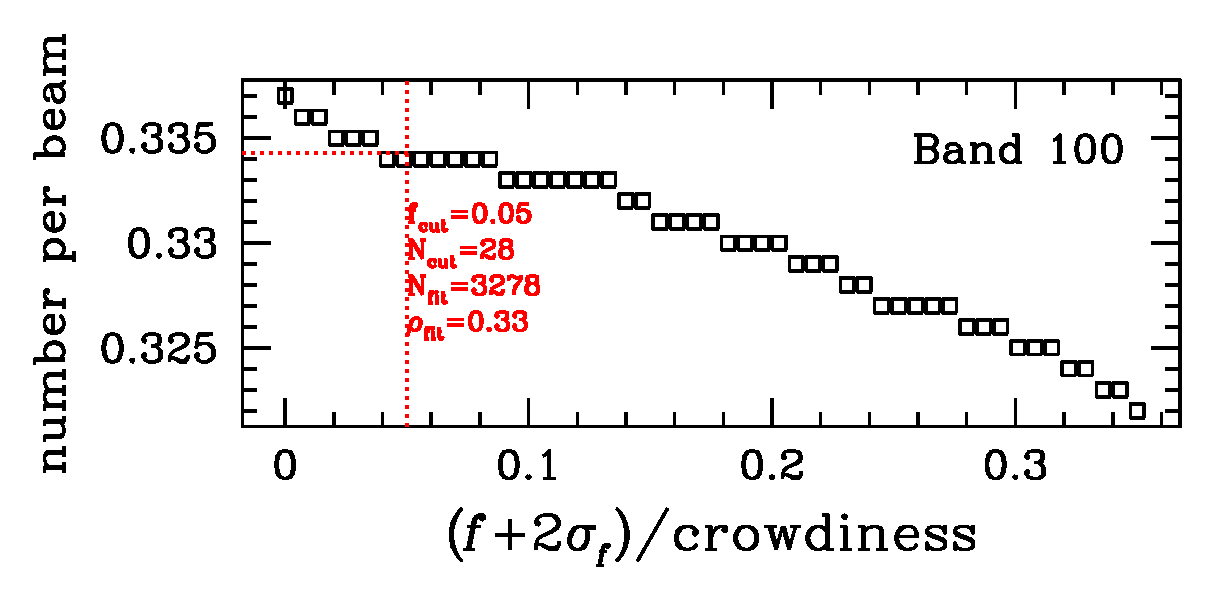
\includegraphics[width=0.85\textwidth]{plot_cutting_flux_100_with_crow}
\end{figure}

We use a $f_{cut} = 0.05$ at band 100, which leads to: 

\indent\hspace{15pt}$\bullet$ 
\textcolor{black!30!white}{Type\_FIT: 3280 out of 3306 sources will be used as prior sources at band 100, while 26 out of 3306 sources are flagged out, which will be not used as prior sources but whose flux will be subtracted from the observed image. $^{obsolete!}$ }
\\
\indent\hspace{15pt}$\bullet$ 
Type\_FIT: 3278 out of 3306 sources will be used as prior sources at band 100, while 28 out of 3306 sources are flagged out, including ID 14834 and 13731. 
\\
\indent\hspace{15pt}$\circ$ 
\textcolor{blue}{DONE: 2015-12: If crowdiness is used for the flagging $(f_{SED}+2\sigma_{f_{SED}})/crowdiness \ge f_{cut}$, then we have 28 out of 3306 flagged out, i.e. two more faint sources: ID 14834 (spec-z 0.202) and 13732 (spec-z 0.079). I have checked that 13732 has a very nearby source 13731, whose old version SED had a bad $\chi^2$, i.e. 100 and 160 measurements were too low while 250 was much higher than the SED best fit. The new flagging will flag out 13732 since band 100, therefore will likely lead to much better SED of 13731. }
\\
\indent\hspace{15pt}$\circ$ 
\textcolor{blue}{DONE: 2015-12: Now we use $(f_{SED}+2\sigma_{f_{SED}})/crowdiness > f_{cut}$ as the criterion to flag out too faint sources.}
\\

\subsection{Faint flux subtraction at band 100}
\label{Band100_Galsub}

We use the SED flux of the flagged faint sources to construct a PSF-modeled image, then subtract it from the original observed image. 

\begin{lstlisting}[language=bash]
./do_Galsub 100 201512 \
-catalog RadioOwenMIPS24_priors_v6_20151221_BeforeBand100.txt \
-fitsname pgh_goodsn_green_Map_v1.0_sci_DL.fits \
-sedpredict SED_predictions_100_201512.txt
\end{lstlisting}

\begin{figure}[H]
	\caption{Faint-source subtraction step at band 100. From left to right: original image, faint-source model image, and faint-source-subtracted image.}
	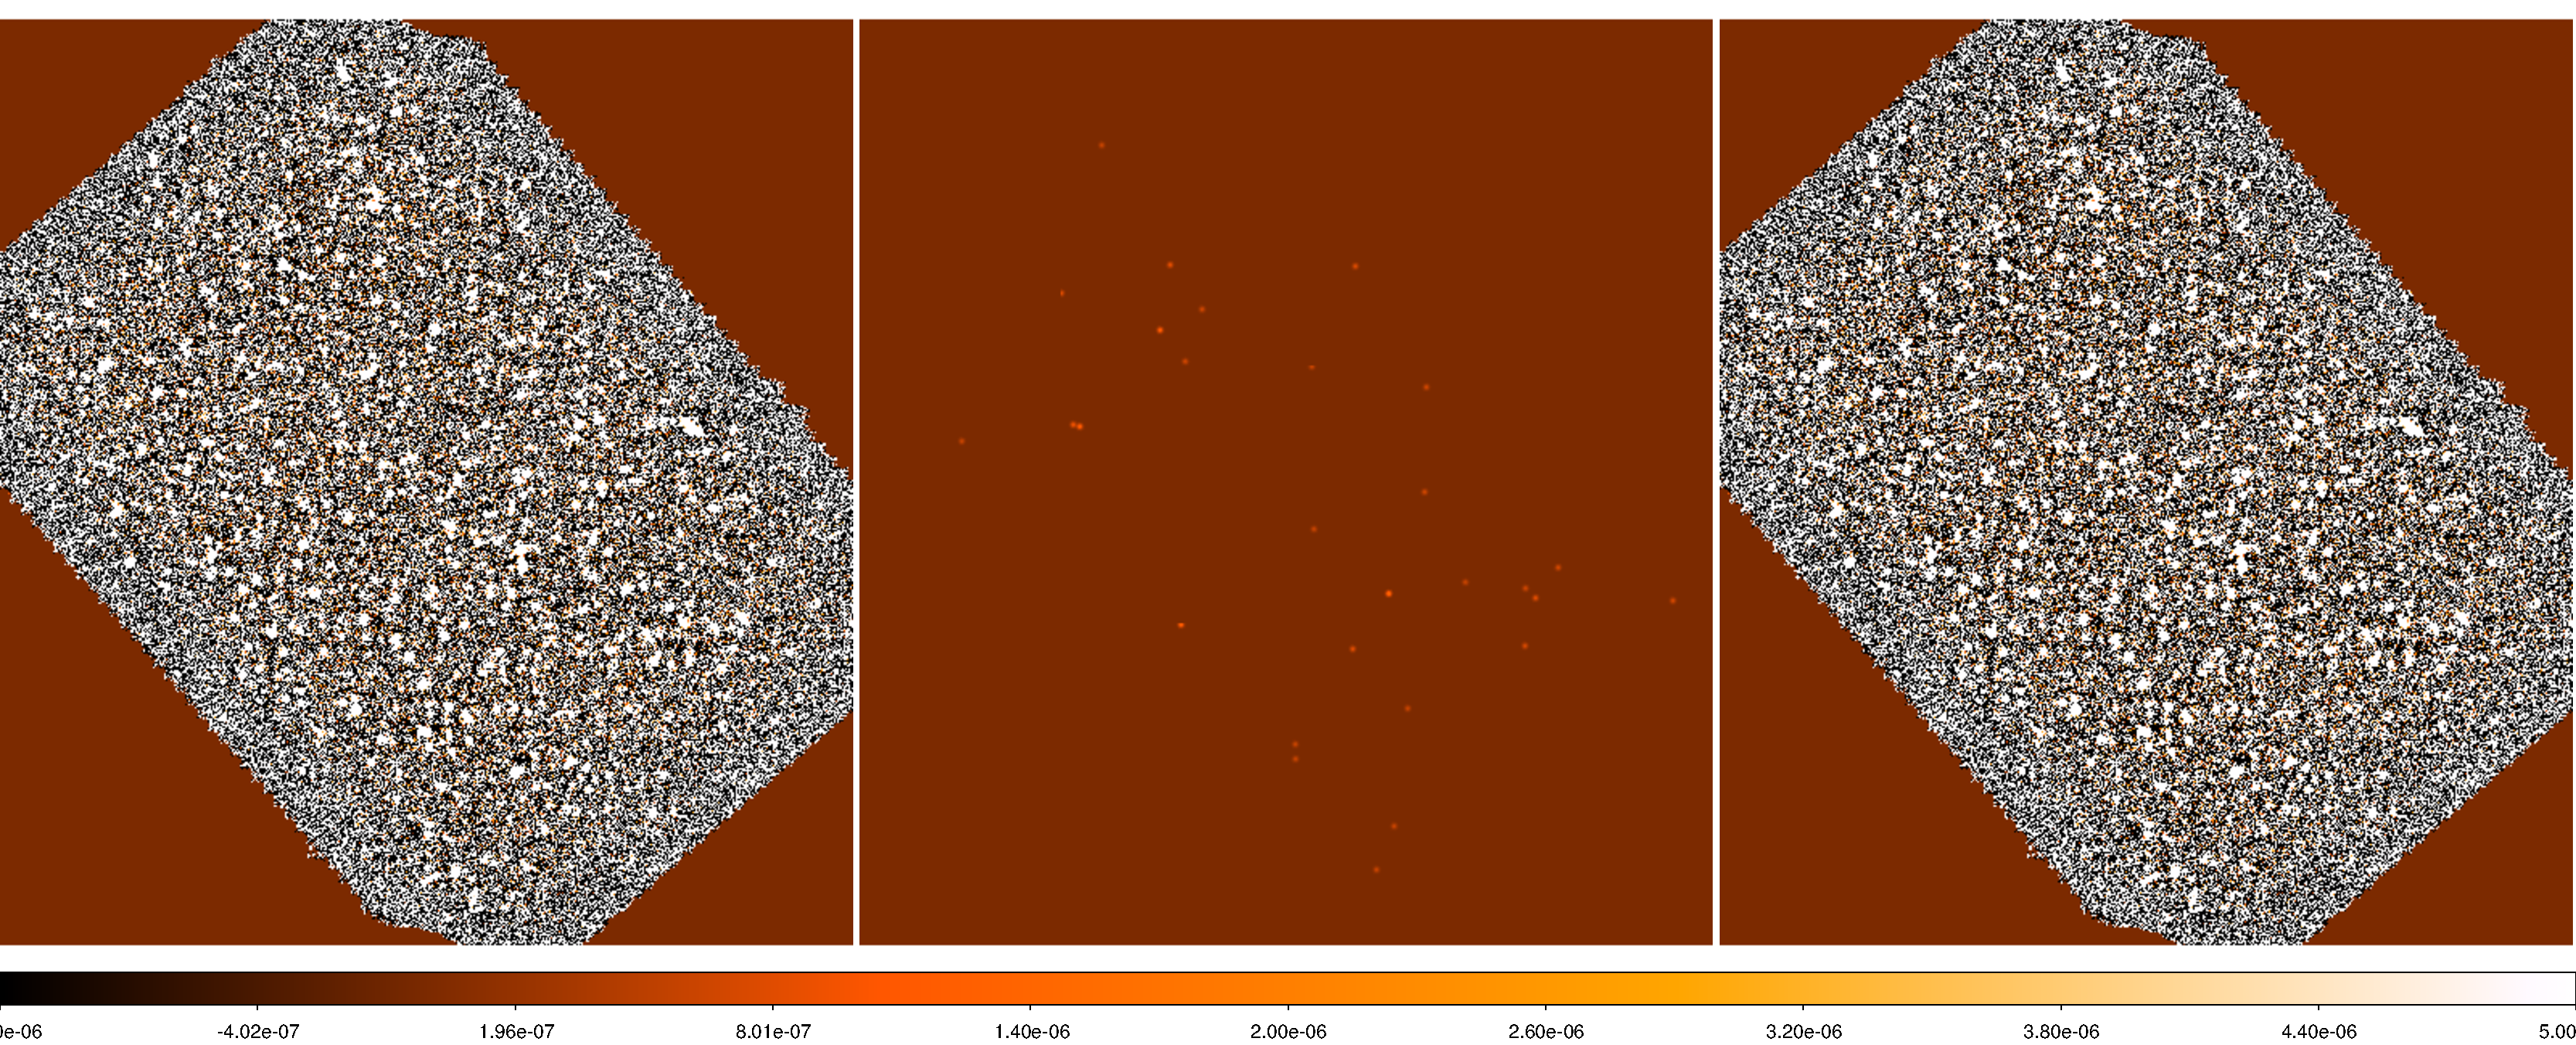
\includegraphics[width=0.9\textwidth]{galfit_100_FIT_goodsn_100_Map_201512_Galsub}
\end{figure}

Using the faint-sources-subtracted image, we perform prior source fitting photometry in the next step. 

\indent\hspace{15pt}$\circ$ 
\textcolor{blue}{Note: Remember to set Xback=0 and fbias=0 while doing the faint-source subtraction.}
\\

\subsection{Galfit photometry at band 100}
\label{Band100_Galfit}

We use supermongo code + galfit software to do the prior source fitting photometry. 

We use the sky background value based on previous simulation results. 
%% But because we use Monte-Carlo simulation to correct flux bias and flux uncertainty in a sophisticated way, the choice of sky background value during the photometry will have very little bias to our final measurements. 

We correct astrometry when needed. For the PACS 100 and 160 images from PEP project, no additional astrometry needs to be corrected. 

But for PACS 100 and 160 images, the flux measurements need high-pass filtering correction: 

\indent\hspace{15pt}$\bullet$ 
If $f_{24}>60$ and $S/N_{24}>3$, we multiply a factor $\times 1.12$ to the measured flux, otherwise $\times 1.19$. 
\\
\indent\hspace{15pt}$\circ$ 
\textcolor{blue}{Note: See ''AGN\_N.sm''.}
\\
\indent\hspace{15pt}$\circ$ 
\textcolor{blue}{Note: Flux bias: Previously we were using a constant flux bias at band 100, 160 and 1160, while a non-linear $\sigma_{f}$-dependent flux bias at band 250, 350 and 500. Now we decide to fully use Monte-Carlo simulation to derive non-linear correction recipes for flux bias correction. See next part. }
\\
\indent\hspace{15pt}$\circ$ 
\textcolor{blue}{Note: Sky background: we have verified that median input minus measured very close to zero.}
\\
\indent\hspace{15pt}$\circ$ 
\textcolor{blue}{Confirmed: For the PACS 100 and 160 images from PEP project, no additional astrometry needs to be corrected.}
\\

\subsection{Residual image at band 100}
\label{Band100_Galres}

We found no obvious additional source from the residual image of band 100. 

\subsection{Monte-Carlo simulation at band 100}
\label{Band100_Galsim}

We simulate one source at each time, and add its PSF-modeled image to the real observed image. Then all sources not flagged out (Type\_FIT=1) are fitted together with the simulated source, and we record the recovered flux and flux uncertainty for the simulated source. The simulated flux, or the input flux $S_{in}$, are compared to the recovered flux, or the output flux $S_{out}$ and the recovered flux uncertainty $\sigma_{S_{out}}$. 

We repeat the procedure 6000 times, so that we have 6000 pairs of $S_{in}$, $S_{out}$, and $\sigma_{S_{out}}$. Statistical analyses are in the following section. 


\subsection{Flux bias and flux uncertainty correction}
\label{Band100_dfcorr}

In one aspect, statistically, the differences between $S_{in}$ and $S_{out}$ should have a mean of 0. Any non-zero mean of the differences $\left<(S_{in}-S_{out})\right>$ is indicating that there have flux bias in the photometry procedure. 

In another aspect, statistically, the flux uncertainty $\sigma_{S_{out}}$ should be consistent with the dispersion of $(S_{in}-S_{out})$. In another word, $(S_{in}-S_{out})/\sigma_{S_{out}}$ should have a shape of Gaussian distribution and a dispersion (Gaussian width $\sigma_{Gaussian}$) of 1.0. 

Based on the above two criterion, we can correct both $S_{out}$ and $\sigma_{S_{out}}$. In the simplest way, we can derive a constant flux bias by taking the mean \textcolor{red}{(TODO: or median?)} $S_{bias}=\left<(S_{in}-S_{out})\right>$, and derive a constant flux uncertainty factor by taking the dispersion ${corr}_{\sigma_{S_{out}}}=\sigma_{\left((S_{in}-S_{out})/\sigma_{S_{out}}\right)}$. However, after the simplest corrections, we find that $\sigma_{S_{out}}$ are still not good enough to match the input and output flux $(S_{in}-S_{out})$ in some individual cases, where the simulated sources either have very high $\sigma_{S_{out}}$, or left over imperfect residual, or are in too crowd fields. 

Therefore, more sophisticated recipes are analyzed here. \textcolor{red}{(TODO: descriptions.)}

\begin{figure}[H]
	\caption{
		\textcolor{red}{(TODO: Band 100 flux bias correction plots:)}
	}
	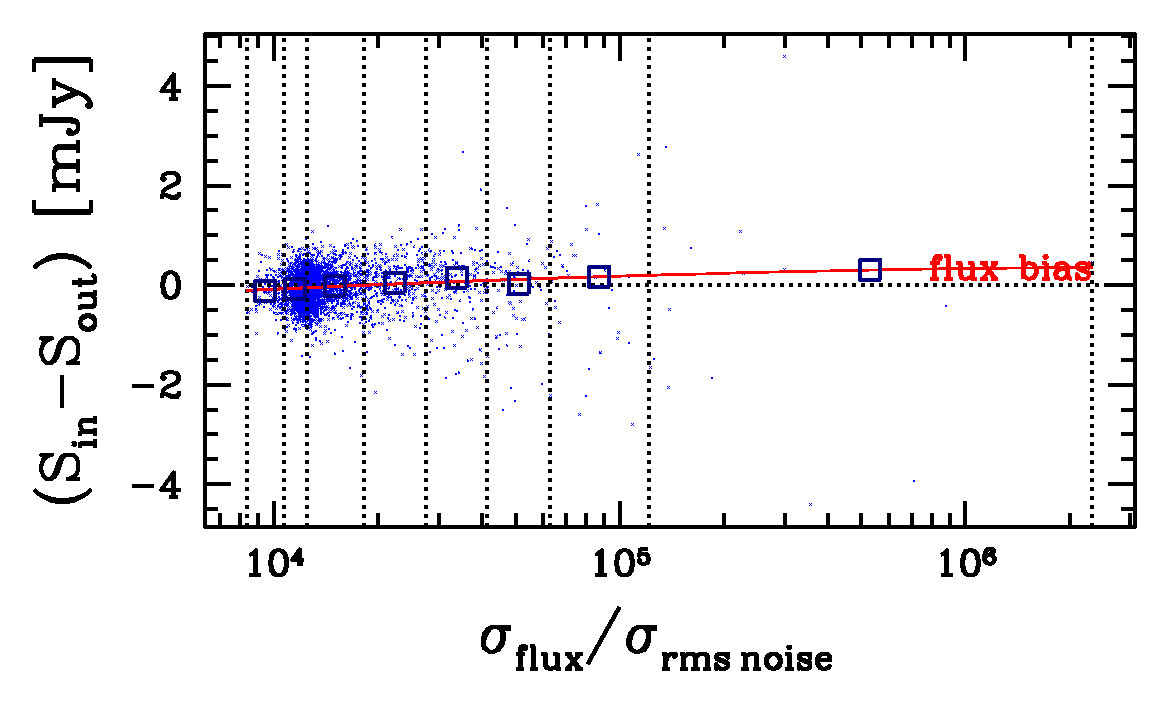
\includegraphics[width=0.65\textwidth]{galsim_100_fbias_1}
	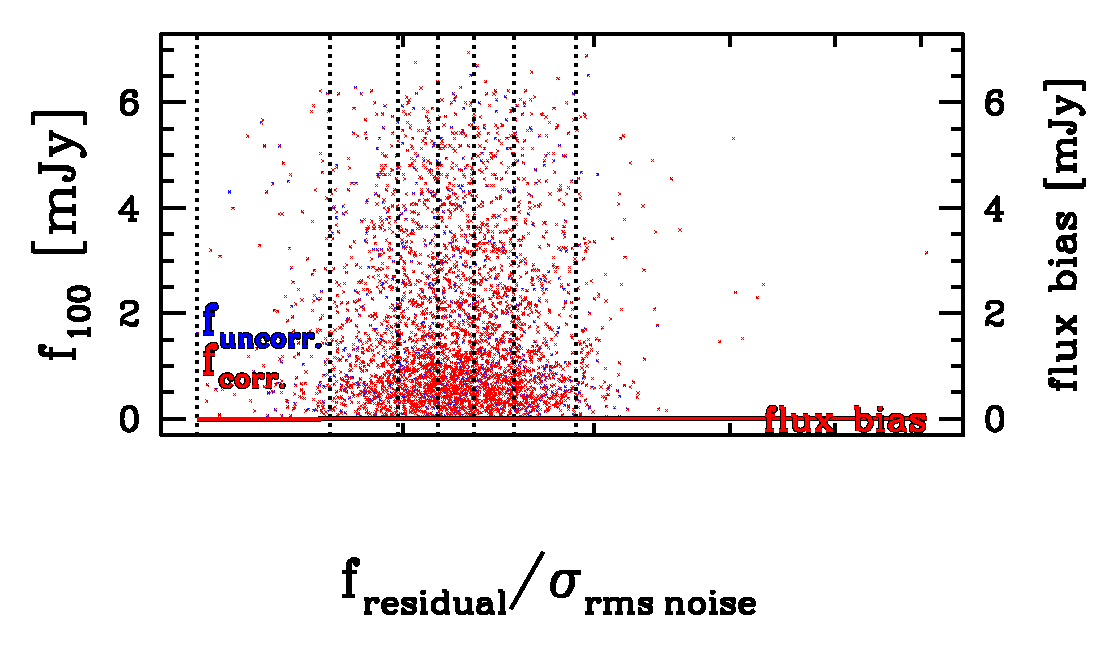
\includegraphics[width=0.65\textwidth]{galsim_100_fbias_2}
	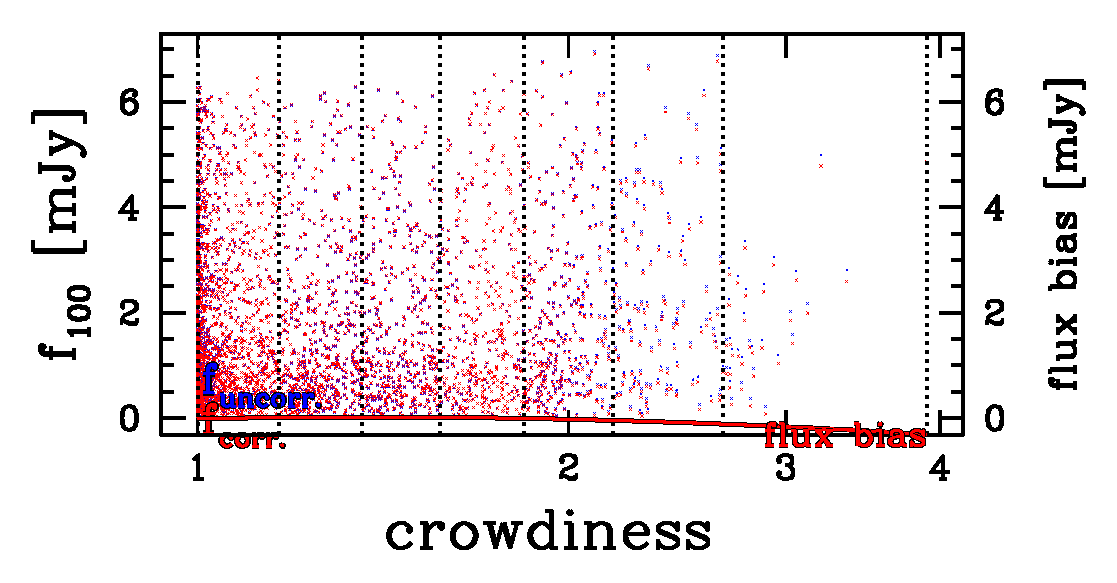
\includegraphics[width=0.65\textwidth]{galsim_100_fbias_3}
\end{figure}

\indent\hspace{15pt}$\circ$ 
\textcolor{blue}{Note: Flux bias corrections: In the plots, the blue data points are uncorrected, while the red ones are corrected. The dashed curve is the flux bias values, which are around 0. A lower than 0 flux bias means that we correct flux bias to be smaller, vice versa. }
\\
\indent\hspace{15pt}$\circ$ 
\textcolor{blue}{Note: Flux bias corrections: Seems the flux bias are very small at band 100. Slightly non-linear trend can be found correlating to $\sigma_{flux}/\sigma_{rms\,noise}$. }
\\

\begin{figure}[H]
	\caption{
		\textcolor{red}{(TODO: Band 100 flux uncertainty correction plots:)}
	}
	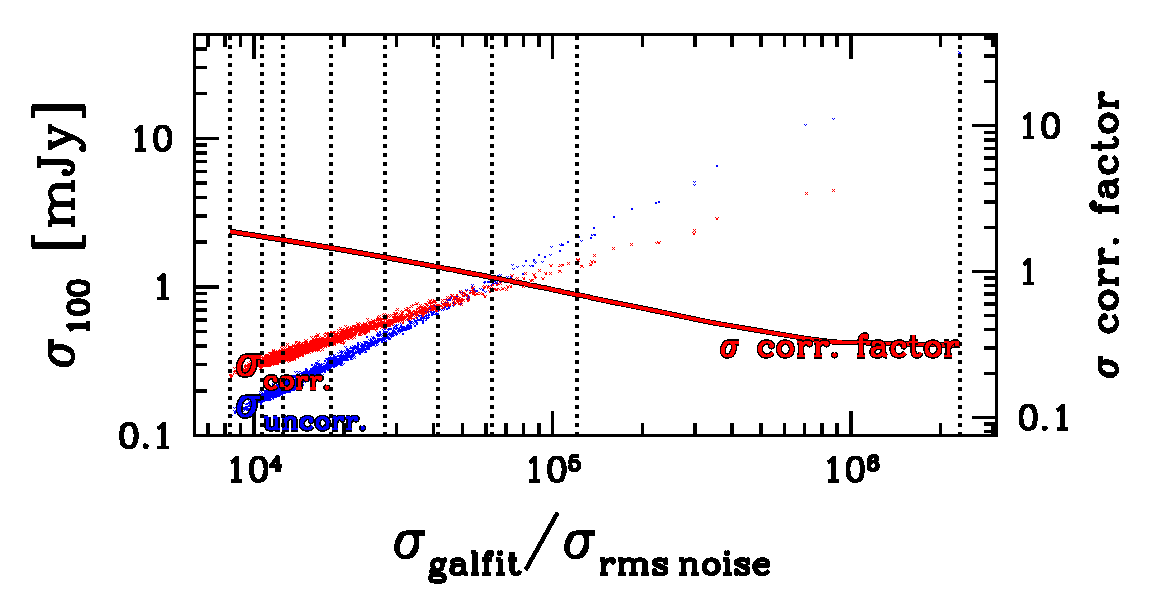
\includegraphics[width=0.65\textwidth]{galsim_100_dfcorr_1}
	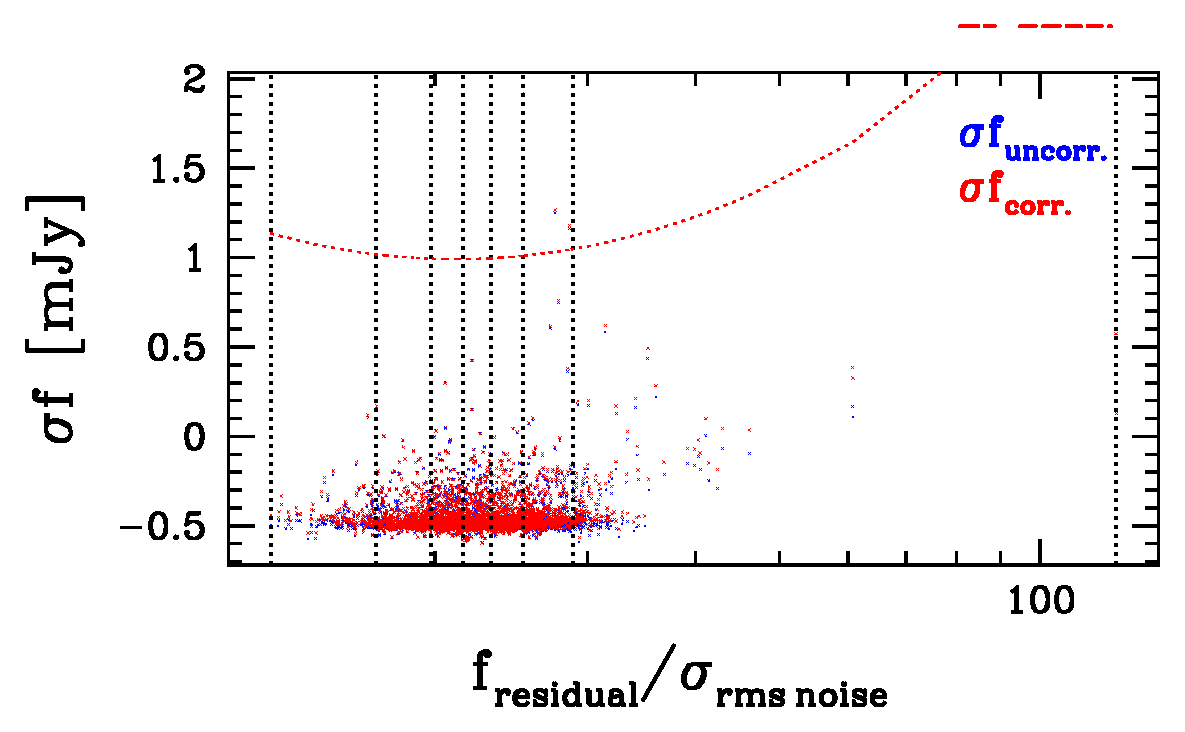
\includegraphics[width=0.65\textwidth]{galsim_100_dfcorr_2}
	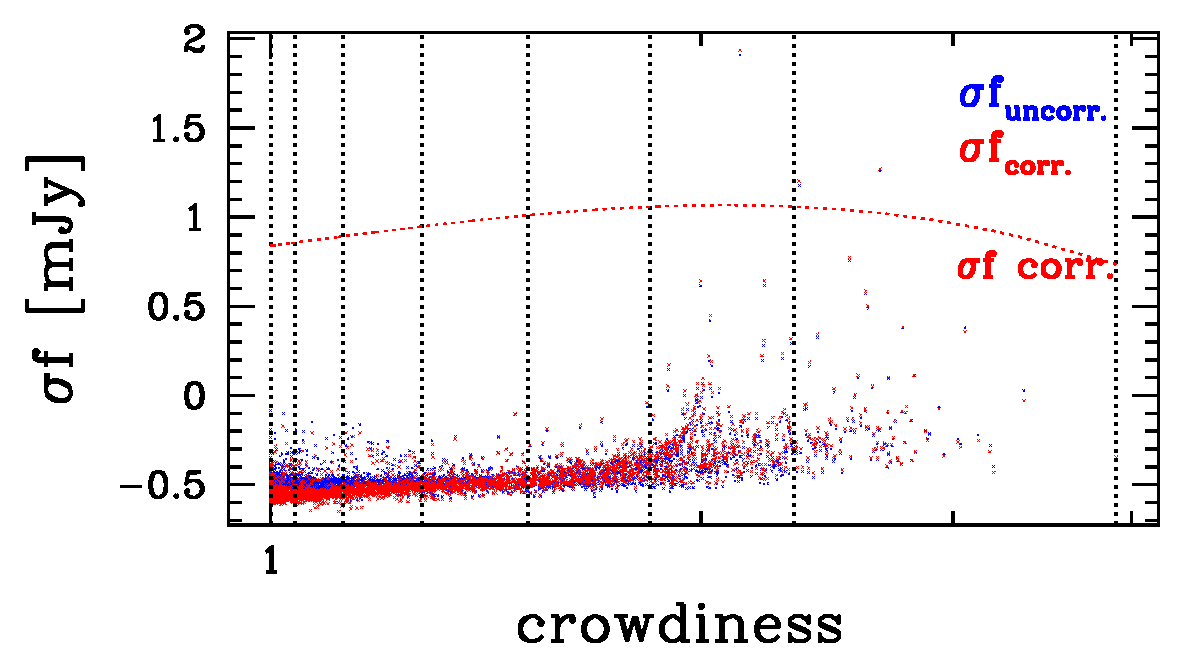
\includegraphics[width=0.65\textwidth]{galsim_100_dfcorr_3}
\end{figure}

\indent\hspace{15pt}$\circ$ 
\textcolor{blue}{Note: Flux uncertainty corrections: In the plots, the blue data points are uncorrected, while the red ones are corrected. The dashed curve is the correction factor values, which are around 1. A lower than 1 corr. factor means that we correct flux uncertainty to be smaller, vice versa. }
\\
\indent\hspace{15pt}$\circ$ 
\textcolor{blue}{Note: Flux uncertainty corrections: Seems performing well. The correlation of $\sigma{f}corr.$ correction factor with $f_{residual}$ is not as prominent as the other two parameters, but it might have stronger correlation at longer wavelength bands.}
\\

%*************************************************************************************
\section{Band 160}

\subsection{SED fitting before band 160}
\label{Band160_Galsed}

At this step, we have obtained new flux measurements and flux uncertainty are band 100. Therefore the SED fitting at this step includes:

\indent\hspace{15pt}$\bullet$ $K_s$
\\
\indent\hspace{15pt}$\bullet$ IRAC 3.6, 4.5, 5.8, 8.0
\\
\indent\hspace{15pt}$\bullet$ IRS PUI 16, MIPS 24
\\
\indent\hspace{15pt}$\bullet$ \textcolor{blue}{PACS 100 $^{new!}$}
\\
\indent\hspace{15pt}$\bullet$ VLA 1.4 GHz (hereafter radio) 
\\

The SED fitting uses the 3 aforementioned parameters, two of which have already been determined in the step \ref{Band100_SED}:

\indent\hspace{15pt}$\bullet$ 
Type\_AGN: 205 radio AGNs, out of 3306 sources in total. 
\\
\indent\hspace{15pt}$\bullet$ 
Type\_SED: 41 pure SB, 891 pure MS, out of 3306 sources in total. 
\\

The 3rd parameter is Type\_FIR, which defines whether the SED will use only FIR (100-1160) data points or not. At this step, the Type\_FIR parameter needs band 100 flux measurements to determine: 

\indent\hspace{15pt}$\bullet$ 
Type\_FIR: If $SNR_{100} \ge 5$, we fit only FIR data points (i.e. only 100 at this step). While $SNR_{100} < 5$, we fit all data points (but radio depends on Type\_AGN).
\\
\indent\hspace{15pt}$\circ$ 
\textcolor{blue}{DONE: 2015-12: Implement SED fitting code, that when Type\_FIR=1, we mask the non-FIR data points by setting the uncertainty values to $10^{10}$, but we still show their measured data points in the SED fitting plot. }
\\
\indent\hspace{15pt}$\circ$ 
\textcolor{blue}{DONE: 2015-12: edaddi: This might be too stringent. We might use $\ge 5$ as a limit, which should be enough to consider the IR as detected by itself.}
\\

Following are two examples of Type\_FIR=1 SEDs: 

\begin{figure}[H]
	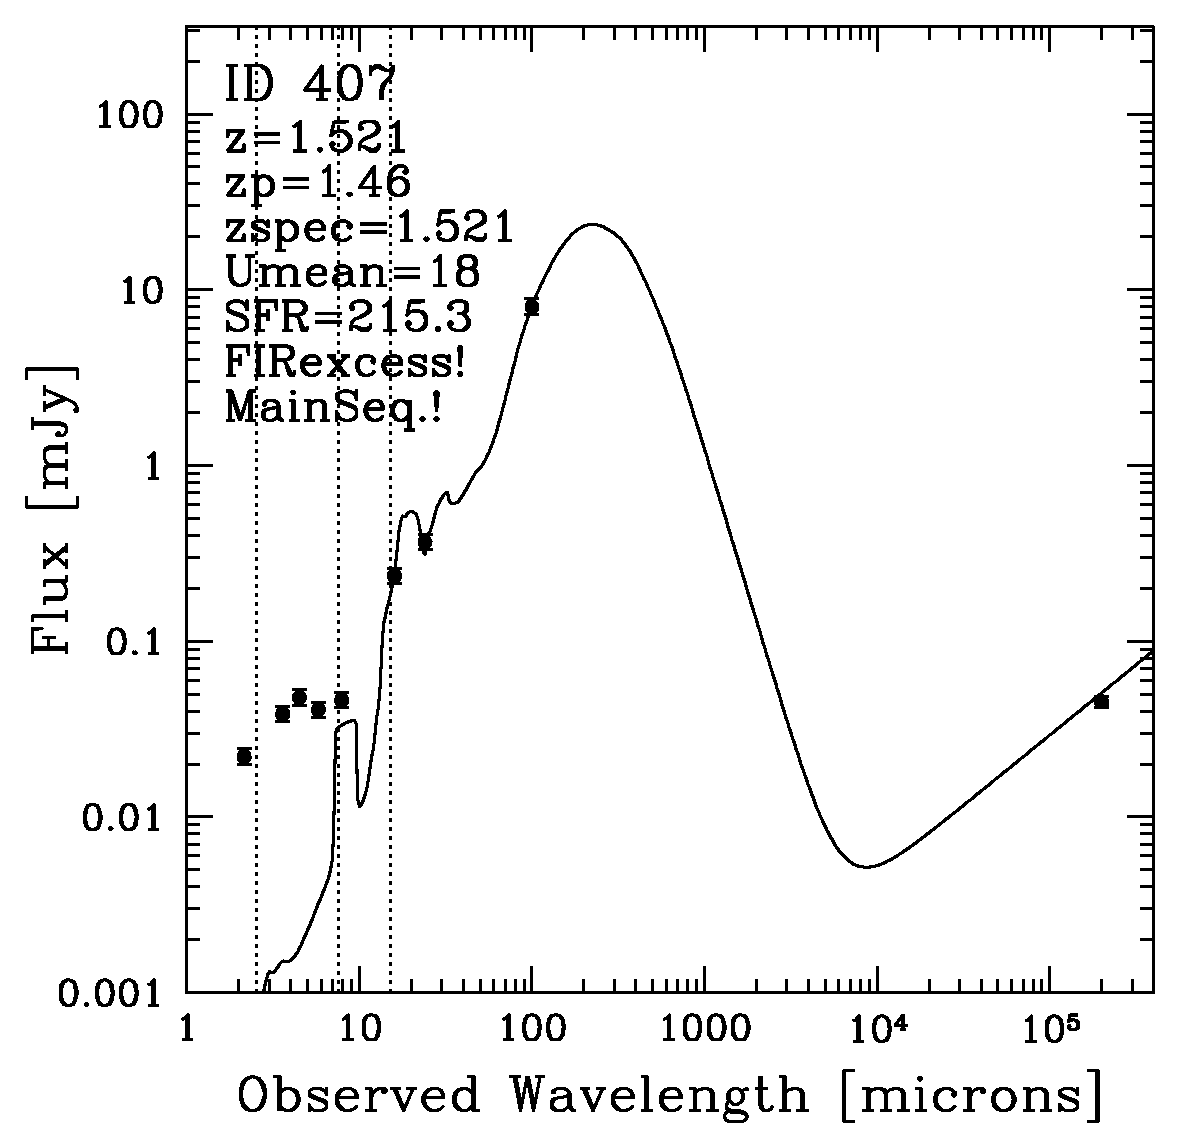
\includegraphics[width=0.65\textwidth]{galsed_160_Plot_SED_407}
\end{figure}

\indent\hspace{15pt}$\circ$ 
\textcolor{blue}{DONE: 2015-12: Found bug in flux residual measuring, which affects the band 100 simulation step. I have redone from that step.}
\\
\indent\hspace{15pt}$\circ$ 
\textcolor{blue}{DONE: 2015-12-21: Found bug in reading the SED prediction file, which affects the band 100 photometry step. I have redone from that step.}
\\
\indent\hspace{15pt}$\circ$ 
\textcolor{blue}{DONE: 2015-12-22: Found bug in supermongo! The supermongo on planer produces different SED best fitting PDF plots, but consistent SED best fitting text files. This is likely because the supermongo on planer was compiled with ''float'' type, while on my local PC it was compiled with ''double'' type. Now I have recompiled supermongo on planer, and the new plots look consistent. The SED best fitting text files seem consistent with my PC results, so no need to redo text files. Therefore, we must follow the same compiling procedure for supermongo as listed in Section \ref{Appendix_Supermongo}.}
\\

\subsection{SED prediction for band 160}

With the best fitting flux at 160um, we can determine which sources to fit and band 160 and which to be flagged out and subtracted: 

\begin{figure}[H]
	\caption{Number of sources kept for fitting per PSF beam area ($\rho_{fit}$) as a function of different $f_{cut}$ at band 160. $\rho_{fit}$ is small at band 160, but we still decide to set a very low $f_{cut}$ to flag out a few sources that are predicted to be too faint or in too crowd environment.}
	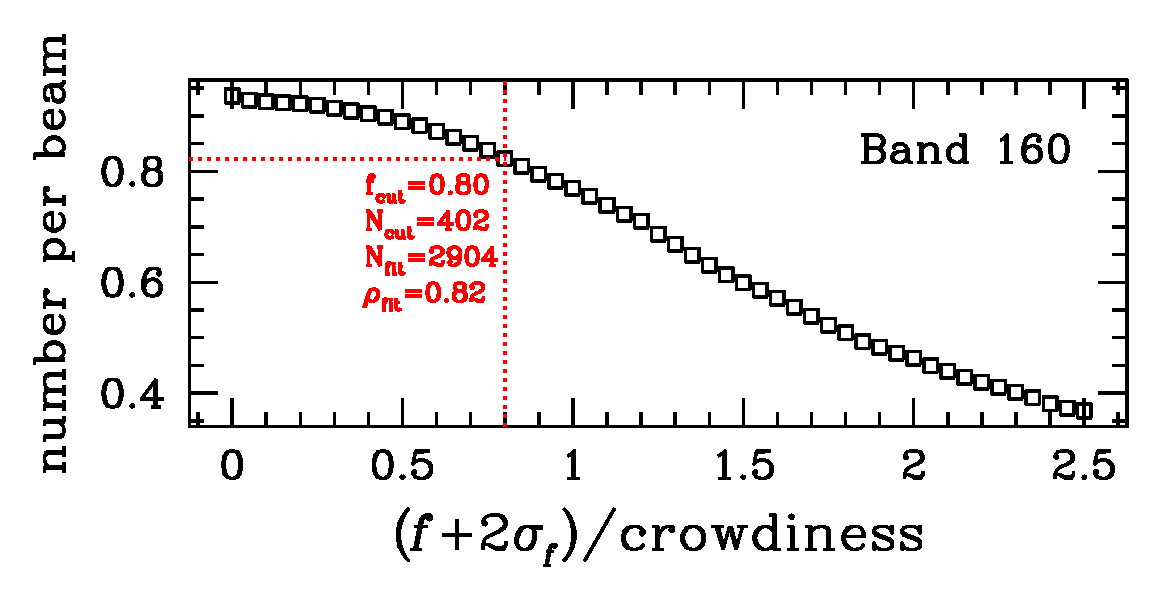
\includegraphics[width=0.85\textwidth]{plot_cutting_flux_160_with_crow}
\end{figure}

\indent\hspace{15pt}$\bullet$ 
Type\_FIT: $(f_{SED,160}+2\sigma_{f_{SED,160}}/crowdiness) \ge 0.80$, 2904 sources will be fit while 402 sources be flagged out. 
\\

\subsection{Faint flux subtraction at band 160}
\label{Band160_Galsub}

We use the SED flux of the flagged faint sources to construct a PSF-modeled image, then subtract it from the original observed image. 

\begin{lstlisting}[language=bash]
./do_Galsub 160 201512 \
-catalog RadioOwenMIPS24_priors_v6_20151221_BeforeBand160.txt \
-fitsname pgh_goodsn_red_Map_v1.0_sci_DL.fits \
-sedpredict SED_predictions_160_201512.txt
\end{lstlisting}

\begin{figure}[H]
	\caption{Faint-source subtraction step at band 160. From left to right: original image, faint-source model image, and faint-source-subtracted image.}
	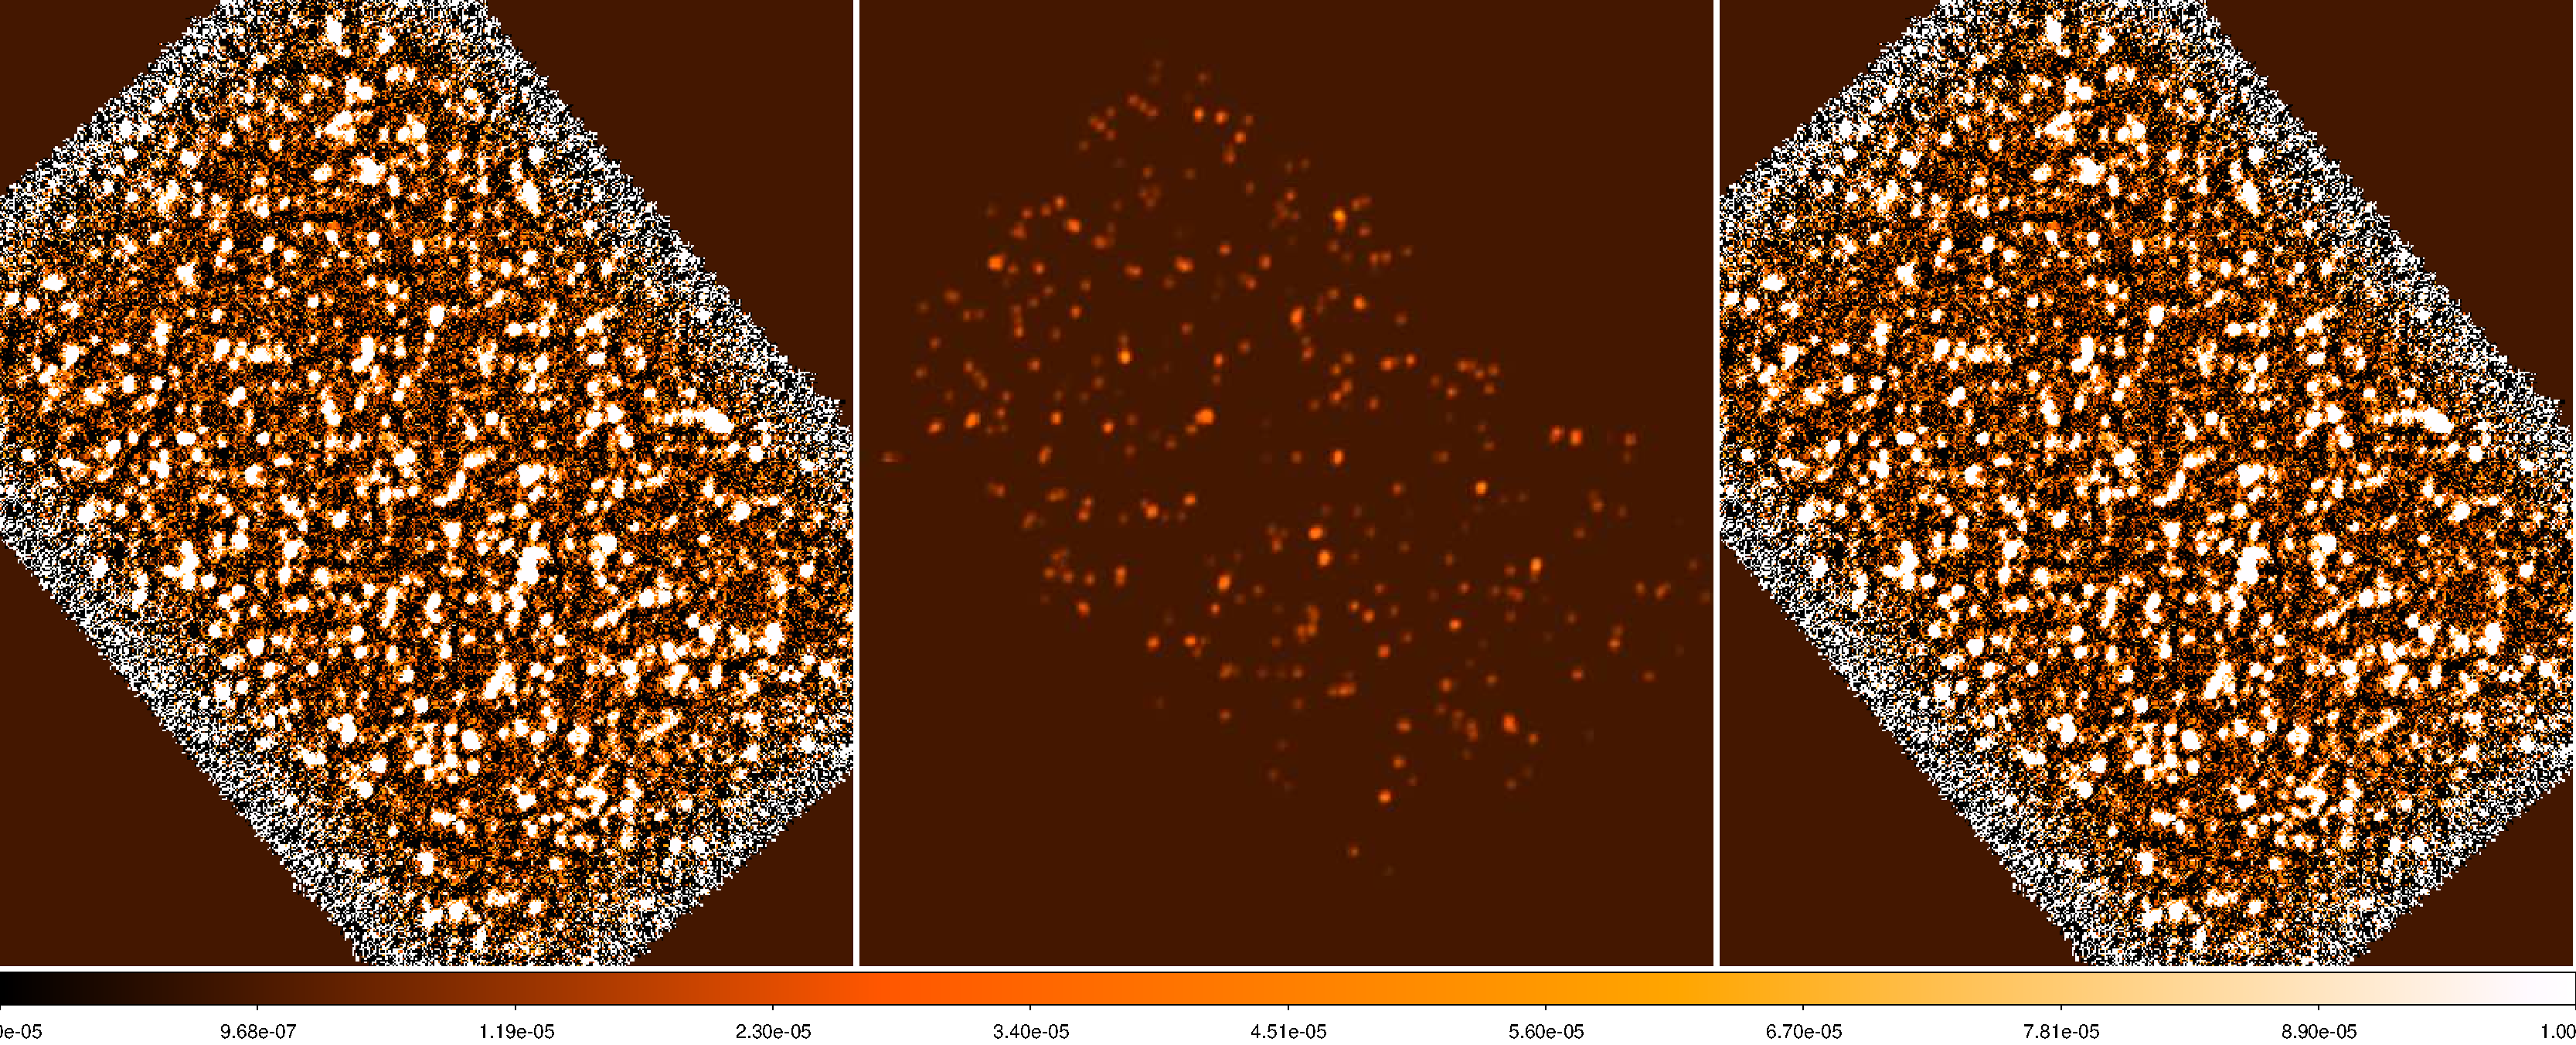
\includegraphics[width=0.9\textwidth]{galfit_160_FIT_goodsn_160_Map_201512_Galsub}
\end{figure}

Using the faint-sources-subtracted image, we perform prior source fitting photometry in the next step. 

\indent\hspace{15pt}$\circ$ 
\textcolor{blue}{Note: Remember to set Xback=0 and fbias=0 while doing the faint-source subtraction.}
\\

\subsection{Galfit photometry at band 160}
\label{Band160_Galfit}

\begin{lstlisting}[language=bash]
./do_Galfit 160 201512 \
-catalog RadioOwenMIPS24_priors_v6_20151221_BeforeBand160.txt \
-fitsname pgh_goodsn_red_Map_v1.0_sci_subfaintDL.fits \
-sedpredict SED_predictions_160_201512.txt
# then run scripts in parallel 
cd boxgalfit; do_GalfitRunqsub
cd ..
# then run postparallel process
./do_Galfit 160 201512 \
-catalog RadioOwenMIPS24_priors_v6_20151221_BeforeBand160.txt \
-fitsname pgh_goodsn_red_Map_v1.0_sci_subfaintDL.fits \
-sedpredict SED_predictions_160_201512.txt \
-postparallel
\end{lstlisting}

\begin{lstlisting}[language=bash]
./do_Galfit 160 201512 \
-catalog RadioOwenMIPS24_priors_v6_20151221_BeforeBand160.txt \
-fitsname pgh_goodsn_red_Map_v1.0_sci_subfaintDL.fits \
-sedpredict SED_predictions_160_201512.txt \
-vary
# then run scripts in parallel 
cd boxgalfit_vary; do_GalfitRunqsub
cd ..
# then run postparallel process
./do_Galfit 160 201512 \
-catalog RadioOwenMIPS24_priors_v6_20151221_BeforeBand160.txt \
-fitsname pgh_goodsn_red_Map_v1.0_sci_subfaintDL.fits \
-sedpredict SED_predictions_160_201512.txt \
-vary -postparallel
\end{lstlisting}

\subsection{Residual image at band 160}
\label{Band160_Galres}

\begin{lstlisting}[language=bash]
cd run_sextractor_160/
idl -e 'do_SExtract_Mask, \
FitsFile="FIT_goodsn_160_Map_201512.fits", \
RmsFile="pgh_goodsn_red_Map_v1.0_rms_DL.fits"'
vim default.sex # set sigma thresholds
sex SExtractor_Signal.fits
# then write additional residual source catalog
# with supermongo code do_sextract_result.sm
gedit do_sextract_result.sm
...
define band 160
set catalog = {"RadioOwenMIPS24_priors_v6_20151221_BeforeBand160.txt"}
set rmsfits24 = {"n_mips_1_s1_v0_37_rms_ED.fits"}
set catalogadd = {"Residual_priors_v6_Band160.txt"}
...
print $(catalogadd) '%-9.0f %12.7f %12.7f %9g\n' \
{_id _ra _de zp_X f24 df24 f16 df16 f100 df100 \
radio eradio _fch1 _dfch1 _fch2 _dfch2 _fch3 _dfch3 _fch4 _dfch4 \
KtotX MassX distX spezX zq source distz idz goodArea}
...
macro read do_sextract_result.sm go
\end{lstlisting}

\textcolor{red}{(TODO: Put Residual Images Here!)}

Then run a second pass \ref{Band160_Galfit}: 

\begin{lstlisting}[language=bash]
./do_Galfit 160 201512 \
-catalog RadioOwenMIPS24_priors_v6_20151221_BeforeBand160.txt \
-catalog-add Residual_priors_v6_Band160.txt \ `\textcolor{blue}{\# ${new!}$}`
-fitsname pgh_goodsn_red_Map_v1.0_sci_subfaintDL.fits \
-sedpredict SED_predictions_160_201512.txt
# then run scripts in parallel 
cd boxgalfit; do_GalfitRunqsub
cd ..
# then run postparallel process
./do_Galfit 160 201512 \
-catalog RadioOwenMIPS24_priors_v6_20151221_BeforeBand160.txt \
-catalog-add Residual_priors_v6_Band160.txt \ `\textcolor{blue}{\# ${new!}$}`
-fitsname pgh_goodsn_red_Map_v1.0_sci_subfaintDL.fits \
-sedpredict SED_predictions_160_201512.txt \
-postparallel
\end{lstlisting}

\subsection{Monte-Carlo simulation at band 160}
\label{Band160_Galsim}

\begin{lstlisting}[language=bash]
# first estimate simulating flux or magnitude range
sm
load astroPhot.sm 
convert_flux2mag goodsn 160 0.40 1.0 # `$1\sigma$` 0.43mJy mag=9
convert_flux2mag goodsn 160 12.0 1.0 # `$30\sigma$` 12mJy mag=5.2
# then run simulation code
./do_Galsim 160 20151201 \
-catalog RadioOwenMIPS24_priors_v6_20151221_BeforeBand160.txt \
-fitsname pgh_goodsn_red_Map_v1.0_sci_subfaintDL.fits \
-sedpredict SED_predictions_160_201512.txt \
-fitincl \
-mag0 5.2 -mag1 9 -nsim 6000 
\end{lstlisting}

\subsection{Flux bias and flux uncertainty correction}
\label{Band160_dfcorr}

\begin{lstlisting}[language=bash]
macro read run_simu_stats_v6.sm run_simu_stats_v6 160
\end{lstlisting}

\begin{figure}[H]
	\caption{
		\textcolor{red}{(TODO: Band 160 flux bias correction plots:)}
	}
	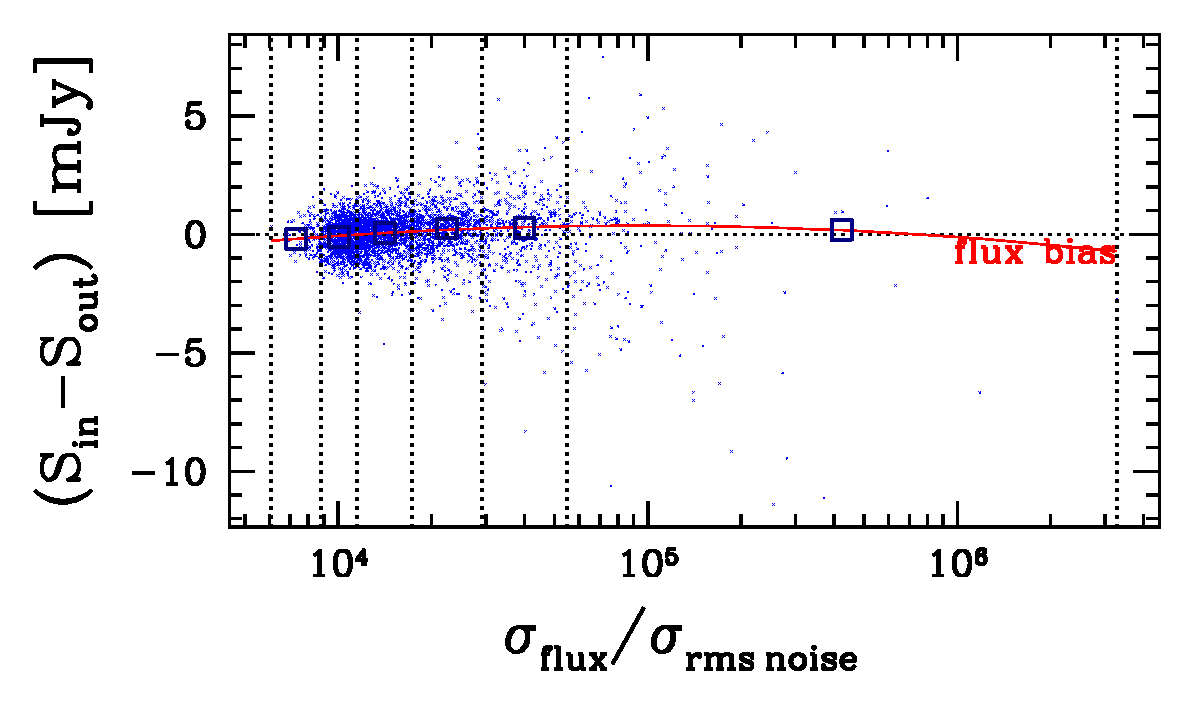
\includegraphics[width=0.65\textwidth]{galsim_160_fbias_1}
	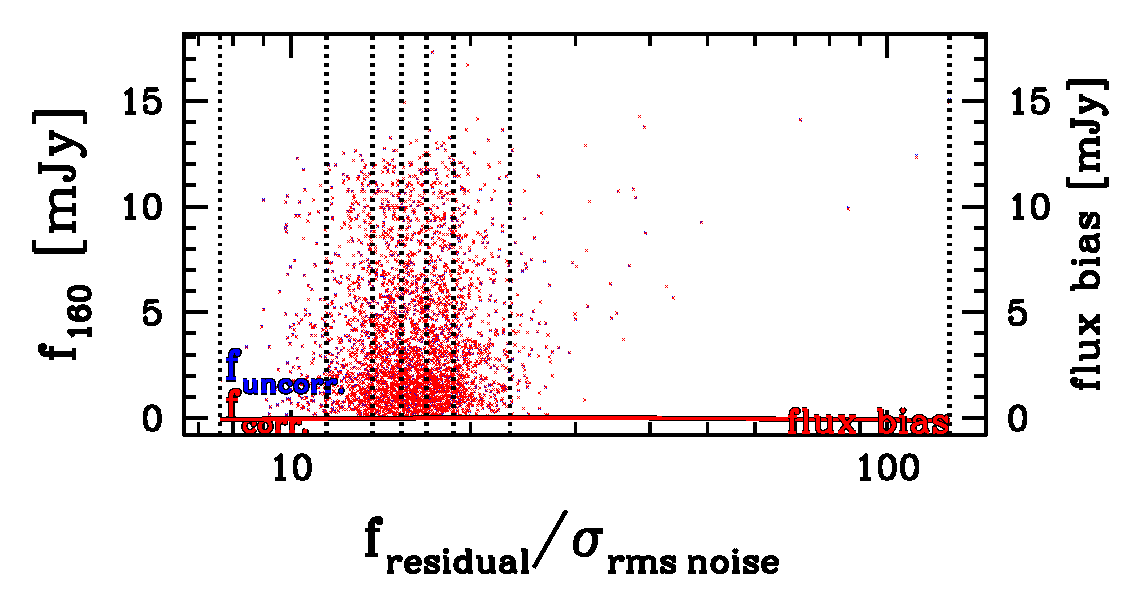
\includegraphics[width=0.65\textwidth]{galsim_160_fbias_2}
	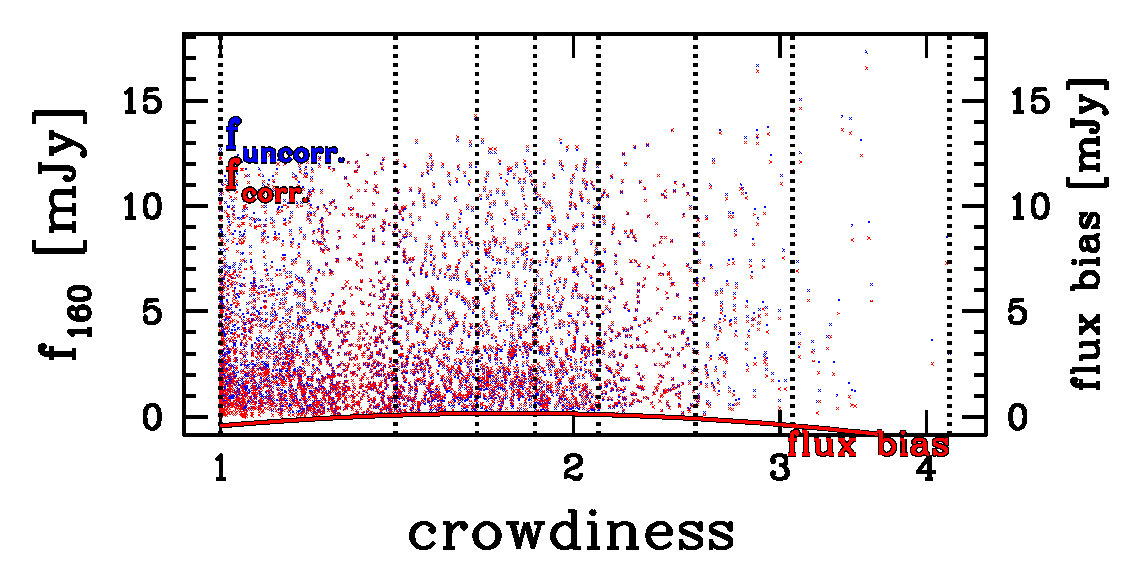
\includegraphics[width=0.65\textwidth]{galsim_160_fbias_3}
\end{figure}

\begin{figure}[H]
	\caption{
		\textcolor{red}{(TODO: Band 160 flux uncertainty correction plots:)}
	}
	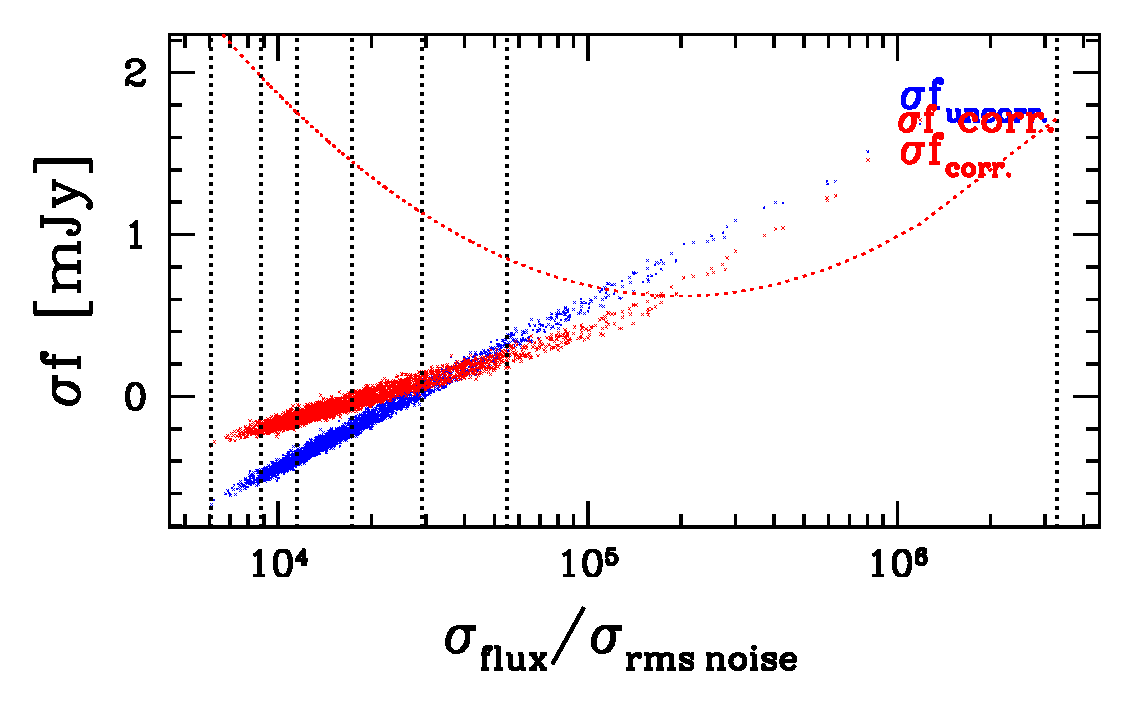
\includegraphics[width=0.65\textwidth]{galsim_160_dfcorr_1}
	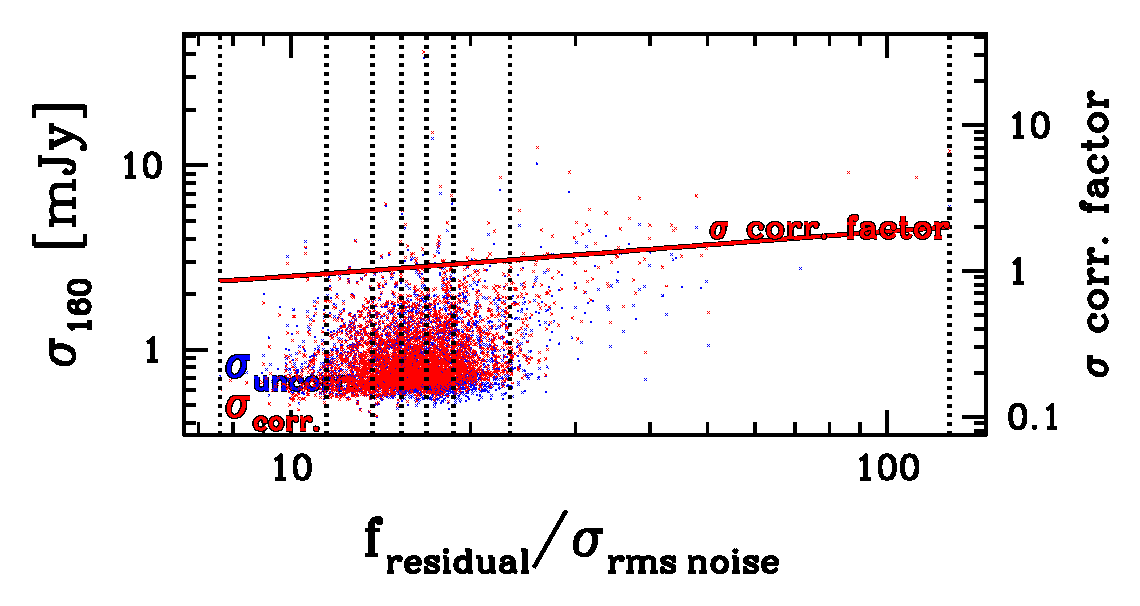
\includegraphics[width=0.65\textwidth]{galsim_160_dfcorr_2}
	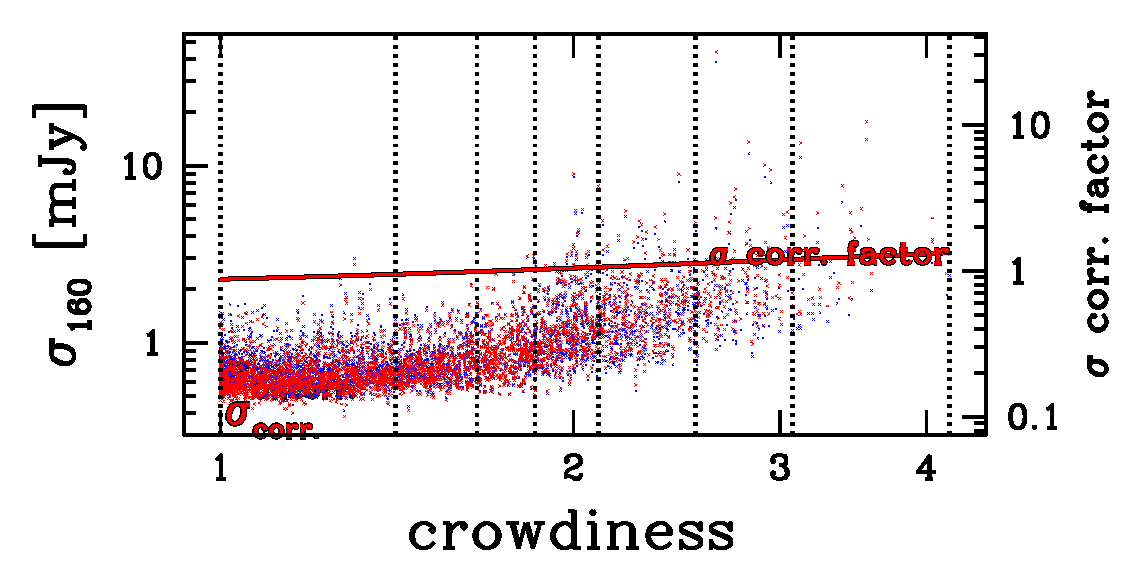
\includegraphics[width=0.65\textwidth]{galsim_160_dfcorr_3}
\end{figure}


\subsection{Update catalog with the measurements of band 160}

\begin{lstlisting}[language=bash]
gedit run_simu_stats_v6.sm
define imax 160
define xdate_galsed 201512
define xdate_galfit 201512
define xdate_galsim 20151201
define xpath_galsed "Galsed_BeforeBand"$imax"_Pass1"
define xpath_galfit "Galfit_Band"$imax"_Pass2"
define xpath_galsim "Galsim_Band"$imax"_Pass1"
set old_catalog = {"RadioOwenMIPS24_priors_v6_20151221_BeforeBand160.txt"}
set new_catalog = {"RadioOwenMIPS24_priors_v6_20151221_BeforeBand250.txt"} \
# found fres -- simu.fits[2] error in previous data, \
# now corrected to [3]. redone Galsim statistics. 
set add_catalog = {"Residual_priors_v6_Band160.txt"}
sm
macro read run_update_catalog_v6.sm run_update_catalog_v6
\end{lstlisting}

%*************************************************************************************

\clearpage

%*************************************************************************************
\section{Band 250}

\subsection{SED fitting before band 250}
\label{Band250_Galsed}

Firstly, we use the Type\_AGN and Type\_SED determined in \ref{Band160_Galsed}:

\indent\hspace{15pt}$\bullet$ 
Type\_AGN: more radio loud AGNs now. Numbers TODO. 
\\
\indent\hspace{15pt}$\bullet$ 
Type\_SED: more MS now. Numbers TODO. 
\\

Then we determine Type\_FIR with the latest 160 measurements:

\indent\hspace{15pt}$\bullet$ 
Type\_FIR: $\sqrt{SNR_{100}^2+SNR_{160}^2} \ge 5$: 940 out of 3320 sources will be fit with only FIR data points. This includes 1 additional residual source. 
\\

Then, \textcolor{blue}{do not forget} to append zeros to coo\_AGN and coo\_SED files for those additional residual sources! Here we have 14 of them, and we set all of their Type\_AGN and Type\_SED to 0, because they do not have radio data point, nor stellar mass measurement. 

\subsection{SED prediction for band 250}
\label{Band250_Galpre}

\begin{lstlisting}[language=bash]
cd Galsed_BeforeBand250_Pass2/do_Type_FIT
gedit do_Type_FIT.sm
define band 250
define fcut$band 1.63
define fmax$band 6.0
set catalog = {"../RadioOwenMIPS24_priors_v6_20151221_BeforeBand250.txt"}
set sedpredict = {"../ResLMTfluxes_priors_v6_20151221_BeforeBand250.txt"}
macro read do_Type_FIT.sm go
Total source number: 3320
Fitting source number: 1528
Subtract source number: 1792
\end{lstlisting}

\begin{figure}[H]
	\caption{Number of sources kept for fitting per PSF beam area ($\rho_{fit}$) as a function of different $f_{cut}$ at band 250.}
	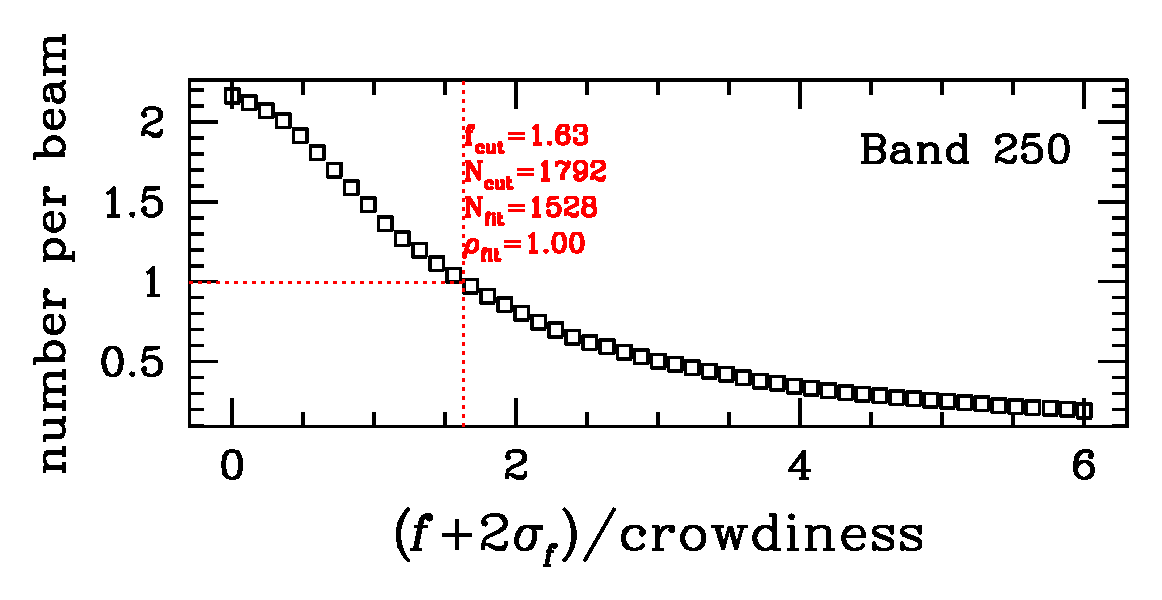
\includegraphics[width=0.85\textwidth]{plot_cutting_flux_250_with_crow}
\end{figure}

\subsection{Faint flux subtraction at band 250}
\label{Band250_Galsub}

We use the SED flux of the flagged faint sources to construct a PSF-modeled image, then subtract it from the original observed image. 

\begin{lstlisting}[language=bash]
./do_Galsub 250 201512 \
-catalog RadioOwenMIPS24_priors_v6_20151221_BeforeBand250.txt \
-fitsname spire250_ima_3p6_v0_100615.fits \
-sedpredict SED_predictions_250_201512.txt
\end{lstlisting}

\begin{figure}[H]
	\caption{Faint-source subtraction step at band 250. From left to right: original image, faint-source model image, and faint-source-subtracted image.}
%	\includegraphics[width=0.9\textwidth]{galfit_250_FIT_goodsn_250_Map_201512_Galsub}
%    TODO
\end{figure}

Using the faint-sources-subtracted image, we perform prior source fitting photometry in the next step. 

\indent\hspace{15pt}$\circ$ 
\textcolor{blue}{Note: Remember to set Xback=0 and fbias=0 while doing the faint-source subtraction.}
\\

\subsection{Galfit photometry at band 250}
\label{Band250_Galfit}

\begin{lstlisting}[language=bash]
./do_Galfit 250 201512 \
-catalog RadioOwenMIPS24_priors_v6_20151221_BeforeBand250.txt \
-fitsname spire250_ima_3p6_v0_100615_subfaintDL.fits \
-sedpredict SED_predictions_250_201512.txt
# then run scripts in parallel 
cd boxgalfit; do_GalfitRunqsub
cd ..
# then run postparallel process
./do_Galfit 250 201512 \
-catalog RadioOwenMIPS24_priors_v6_20151221_BeforeBand250.txt \
-fitsname spire250_ima_3p6_v0_100615_subfaintDL.fits \
-sedpredict SED_predictions_250_201512.txt \
-postparallel
\end{lstlisting}

\subsection{Residual image at band 250}
\label{Band250_Galres}

\begin{lstlisting}[language=bash]
cd run_sextractor_250/
idl -e 'do_SExtract_Mask, \
FitsFile="FIT_goodsn_250_Map_201512.fits", \
RmsFile="spire250_rms_3p6_v0_100615.fits"'
vim default.sex # set sigma thresholds
sex SExtractor_Signal.fits
# then write additional residual source catalog
# with supermongo code do_sextract_result.sm
gedit do_sextract_result.sm
...
define band 250
set catalog = {"RadioOwenMIPS24_priors_v6_20151221_BeforeBand250.txt"}
set rmsfits24 = {"n_mips_1_s1_v0_37_rms_ED.fits"}
set catalogadd = {"Residual_priors_v6_Band250.txt"}
...
print $(catalogadd) '%-9.0f %12.7f %12.7f %9g\n' \
{_id _ra _de zp_X f24 df24 f16 df16 f100 df100 f160 df160 \
radio eradio _fch1 _dfch1 _fch2 _dfch2 _fch3 _dfch3 _fch4 _dfch4 \
KtotX MassX distX spezX zq source distz idz goodArea}
...
macro read do_sextract_result.sm go
\end{lstlisting}

\textcolor{red}{(TODO: Put Residual Images Here!)}

Then run a second pass \ref{Band250_Galfit}: 

\begin{lstlisting}[language=bash]
./do_Galfit 250 201512 \
-catalog RadioOwenMIPS24_priors_v6_20151221_BeforeBand250.txt \
-catalog-add Residual_priors_v6_Band250.txt \ `\textcolor{blue}{\# ${new!}$}`
-fitsname spire250_ima_3p6_v0_100615_subfaintDL.fits \
-sedpredict SED_predictions_250_201512.txt
# then run scripts in parallel 
cd boxgalfit; do_GalfitRunqsub
cd ..
# then run postparallel process
./do_Galfit 250 201512 \
-catalog RadioOwenMIPS24_priors_v6_20151221_BeforeBand250.txt \
-catalog-add Residual_priors_v6_Band250.txt \ `\textcolor{blue}{\# ${new!}$}`
-fitsname spire250_ima_3p6_v0_100615_subfaintDL.fits \
-sedpredict SED_predictions_250_201512.txt \
-postparallel
\end{lstlisting}

\subsection{Monte-Carlo simulation at band 250}
\label{Band250_Galsim}

\begin{lstlisting}[language=bash]
# first estimate simulating flux or magnitude range
sm
load astroPhot.sm 
convert_flux2mag goodsn 250 1.90 1.0 # 250um 1-sigma 1.98mJy -> mag=3.069
convert_flux2mag goodsn 250 57.0 1.0 # -> mag=-0.62
# then run the simulation code
./do_Galsim 250 20151201 \
-catalog RadioOwenMIPS24_priors_v6_20151221_BeforeBand250.txt \
-fitsname spire250_ima_3p6_v0_100615_subfaintDL.fits \
-sedpredict SED_predictions_250_201512.txt \
-fitincl -mag0 -0.62 -mag1 3.07 -nsim 6000 
./do_Galsim 250 20151201 \
-catalog RadioOwenMIPS24_priors_v6_20151221_BeforeBand250.txt \
-fitsname spire250_ima_3p6_v0_100615_subfaintDL.fits \
-sedpredict SED_predictions_250_201512.txt \
-fitincl -mag0 -0.62 -mag1 3.07 -nsim 6000 \
-postparallel
\end{lstlisting}

\subsection{Flux bias and flux uncertainty correction}
\label{Band250_dfcorr}

\begin{lstlisting}[language=bash]
gedit run_simu_stats_v6.sm
sm
macro read run_simu_stats_v6.sm run_simu_stats_v6 250
\end{lstlisting}

\begin{figure}[H]
	\caption{
		\textcolor{red}{(TODO: Band 250 flux bias correction plots:)}
	}
	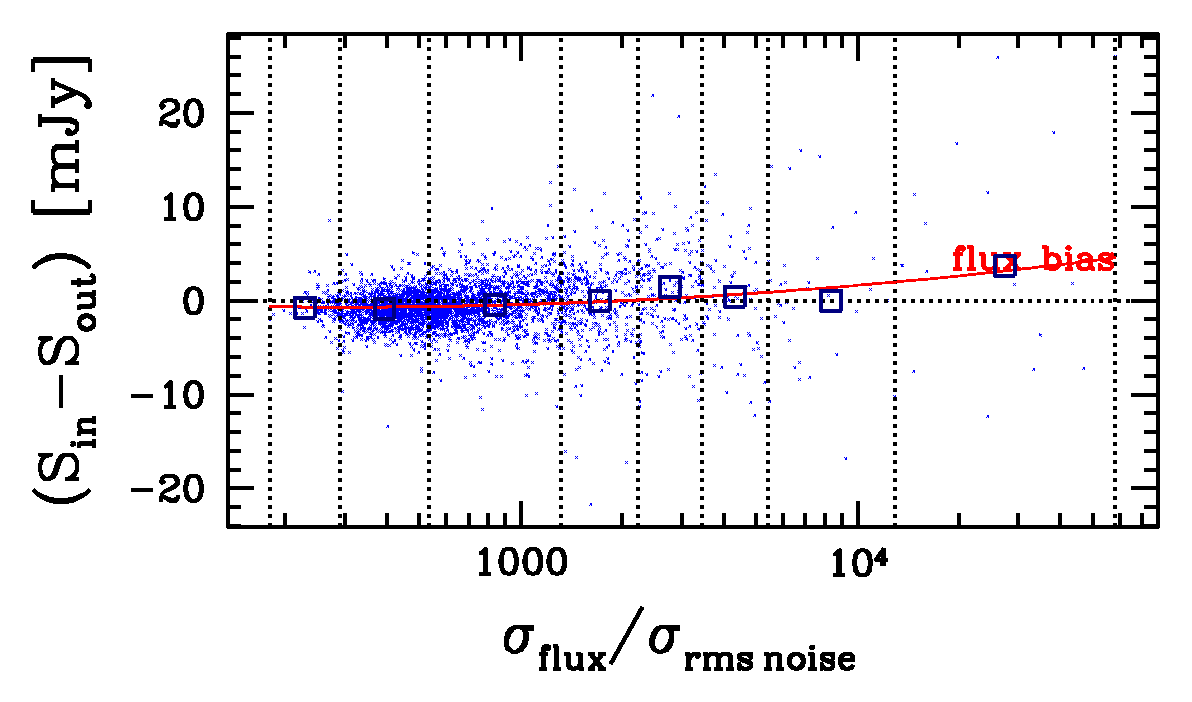
\includegraphics[width=0.65\textwidth]{galsim_250_fbias_1}
	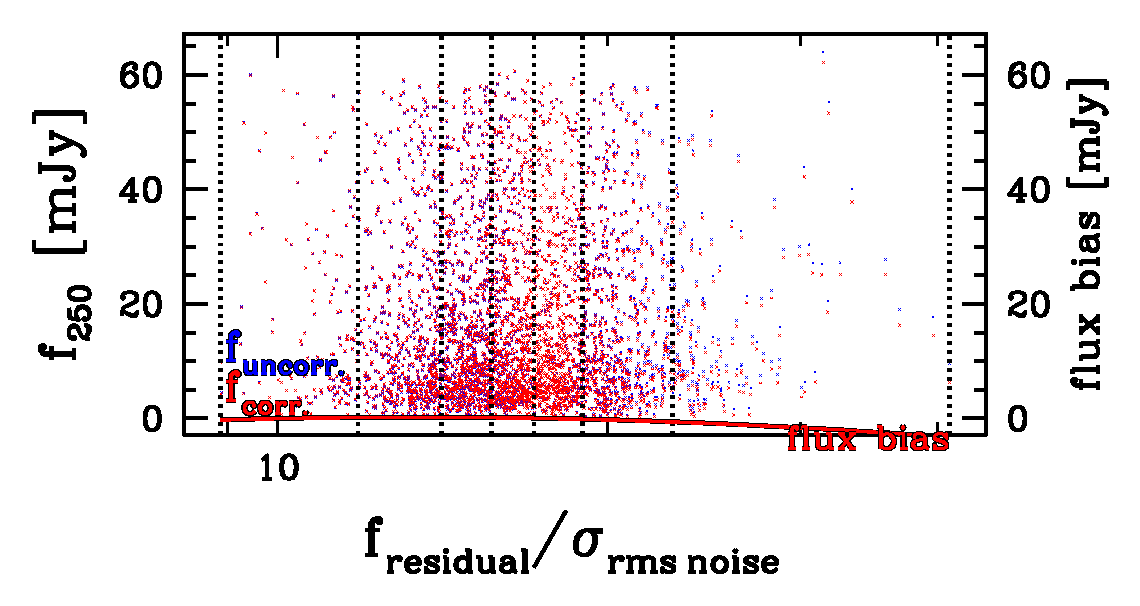
\includegraphics[width=0.65\textwidth]{galsim_250_fbias_2}
	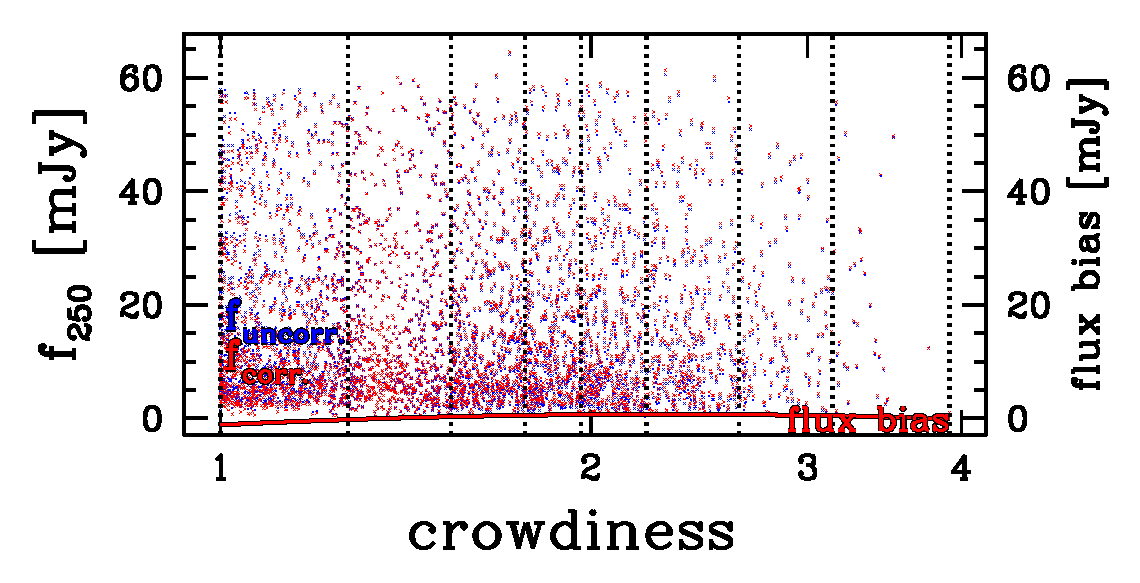
\includegraphics[width=0.65\textwidth]{galsim_250_fbias_3}
\end{figure}

\begin{figure}[H]
	\caption{
		\textcolor{red}{(TODO: Band 250 flux uncertainty correction plots:)}
	}
	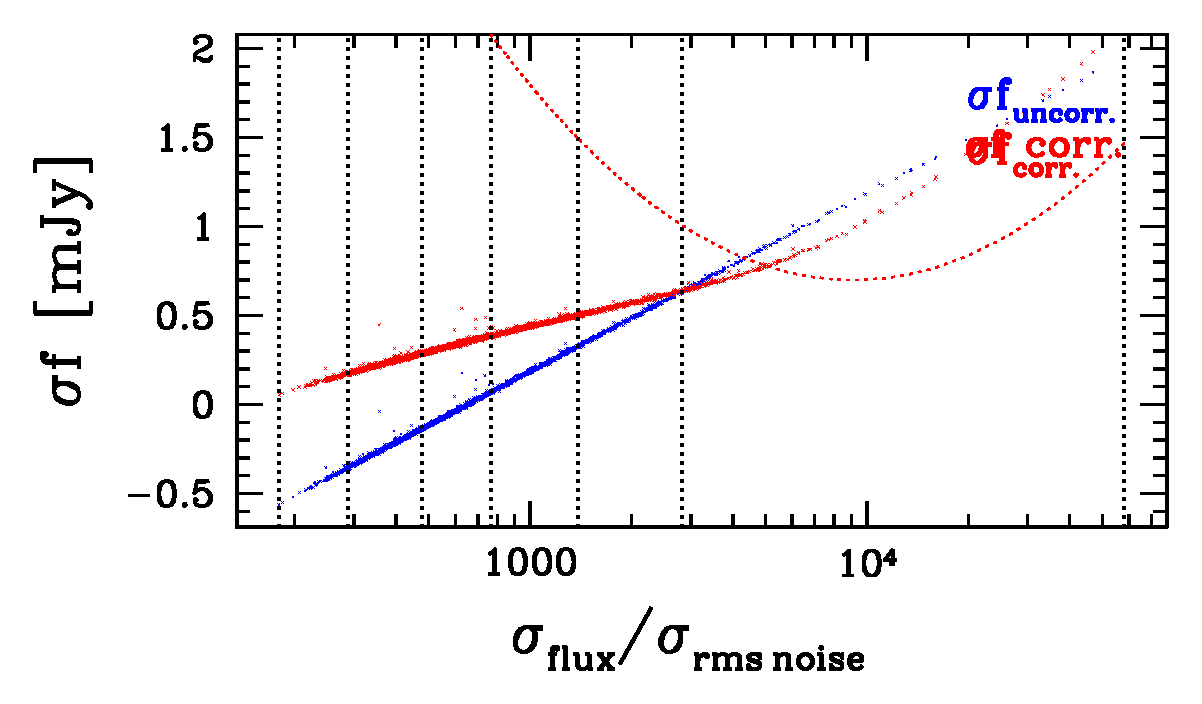
\includegraphics[width=0.65\textwidth]{galsim_250_dfcorr_1}
	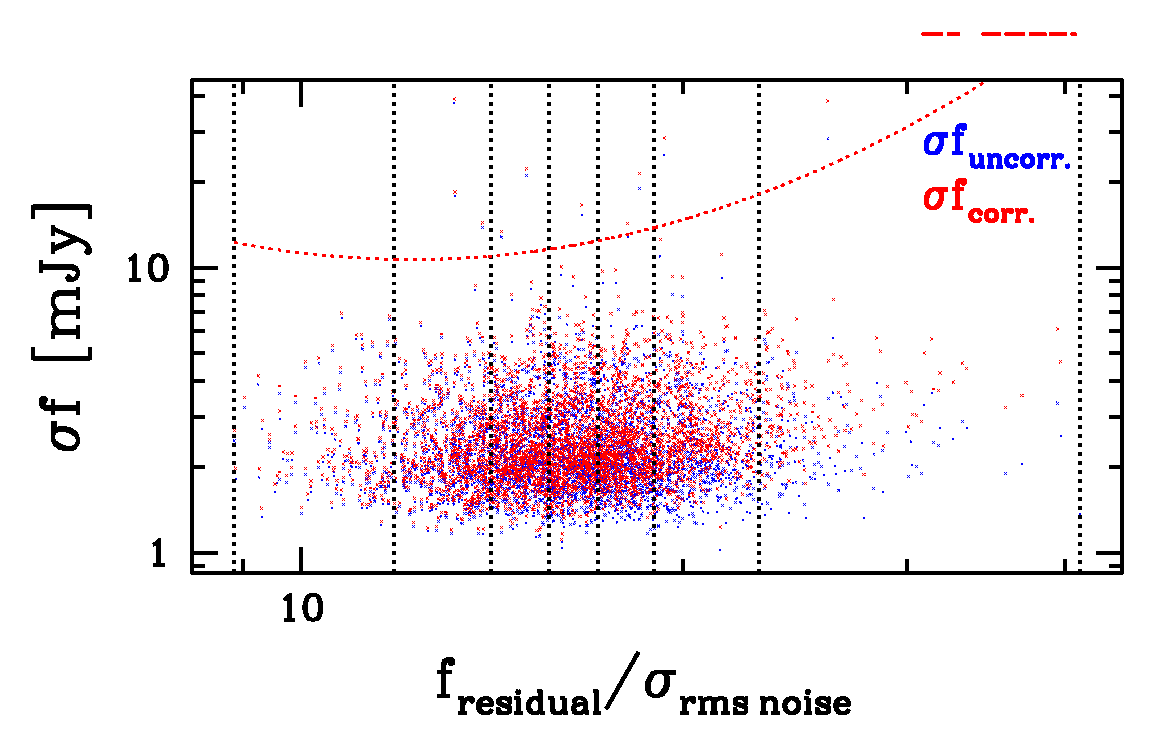
\includegraphics[width=0.65\textwidth]{galsim_250_dfcorr_2}
	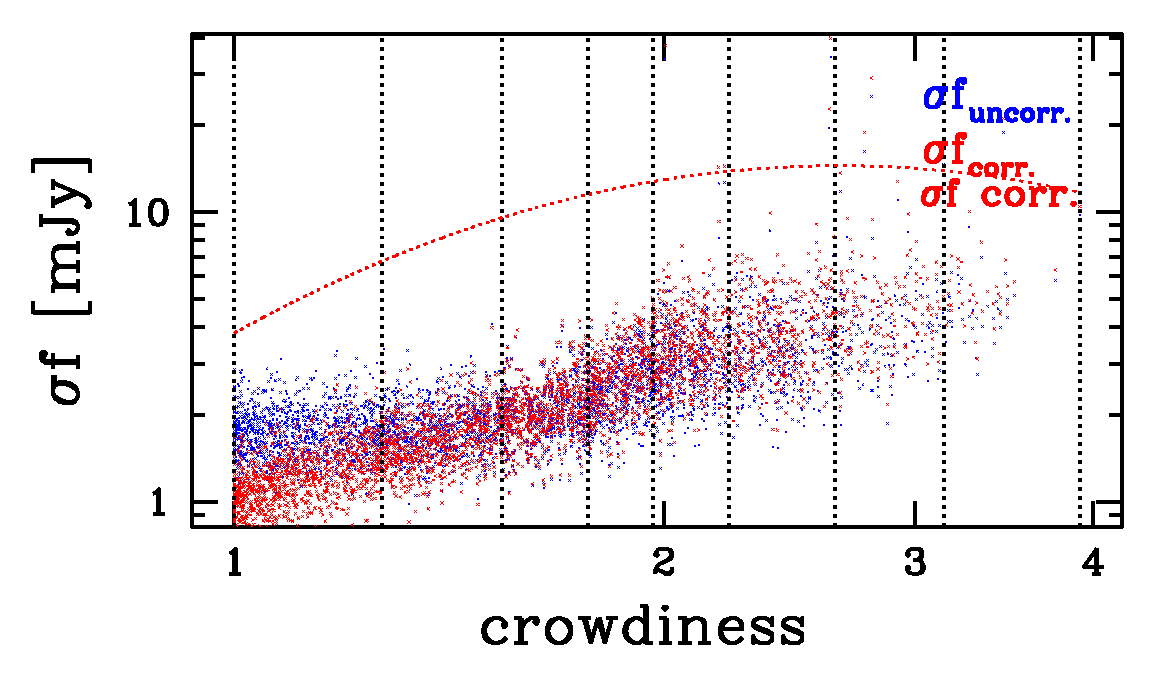
\includegraphics[width=0.65\textwidth]{galsim_250_dfcorr_3}
\end{figure}

\subsection{Update catalog with new corrected measurements}

\begin{lstlisting}[language=bash]
gedit run_update_catalog_v6.sm
define xdate_galsed 201512
define xdate_galfit 201512
define xdate_galsim 20151201
define xpath_galsed "Galsed_BeforeBand"$imax"_Pass2"
define xpath_galfit "Galfit_Band"$imax"_Pass2"
define xpath_galsim "Galsim_Band"$imax"_Pass1"
set old_catalog = {"RadioOwenMIPS24_priors_v6_20151221_BeforeBand250.txt"}
set new_catalog = {"RadioOwenMIPS24_priors_v6_20151221_BeforeBand350.txt"}
set add_catalog = {"Residual_priors_v6_Band250.txt"}
sm
macro read run_update_catalog_v6.sm run_update_catalog_v6 250
\end{lstlisting}

%*************************************************************************************

\clearpage

%*************************************************************************************
\section{Band 350}

\subsection{SED fitting before band 350}
\label{Band350_Galsed}

Firstly, we use the Type\_AGN and Type\_SED determined in \ref{Band250_Galsed}:

\indent\hspace{15pt}$\bullet$ 
Type\_AGN: more radio loud AGNs now. Numbers TODO. 
\\
\indent\hspace{15pt}$\bullet$ 
Type\_SED: more MS now. Numbers TODO. 
\\
\indent\hspace{15pt}$\circ$ 
\textcolor{blue}{Note: \textcolor{blue}{do not forget} to append zeros for additional sources found in the residual image of 250.}
\\

Then we determine Type\_FIR with the latest 250 measurements:

\indent\hspace{15pt}$\bullet$ 
Type\_FIR: $\sqrt{SNR_{100}^2+SNR_{160}^2+SNR_{250}^2} \ge 5$: 1047 out of 3334 sources will be fit with only FIR data points. This includes the additional residual sources found on 160 and 250 residual images. 
\\

Run SED fitting code on planer:

\begin{lstlisting}[language=bash]
scp Galsed_BeforeBand350_Pass1_BeforeFitting_20151223.tar.gz \
dliu@hubble.extra.cea.fr:/dsm/upgal/data/dliu/daddi_goodsn_2015/
cd /dsm/upgal/data/dliu/daddi_goodsn_2015/Galsed_BeforeBand350_Pass1/
./do_GalsedRunqsub
\end{lstlisting}

\subsection{SED prediction for band 350}
\label{Band350_Galpre}

\begin{lstlisting}[language=bash]
cd Galsed_BeforeBand350_Pass2/do_Type_FIT
gedit do_Type_FIT.sm
define band 350
define fcut$band 1.55
define fmax$band 6.0
set catalog = {"../RadioOwenMIPS24_priors_v6_20151221_BeforeBand350.txt"}
set sedpredict = {"../ResLMTfluxes_priors_v6_20151221_BeforeBand350.txt"}
macro read do_Type_FIT.sm go
Total source number: 3334
Fitting source number: 817
Subtract source number: 2517
\end{lstlisting}

\begin{figure}[H]
	\caption{Number of sources kept for fitting per PSF beam area ($\rho_{fit}$) as a function of different $f_{cut}$ at band 350.}
	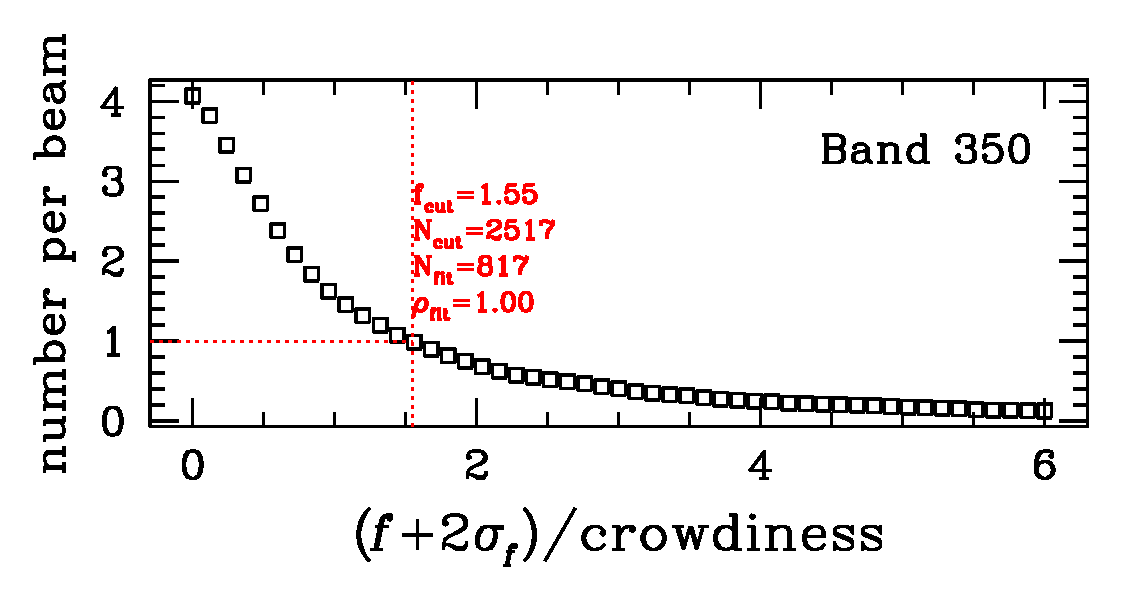
\includegraphics[width=0.85\textwidth]{plot_cutting_flux_350_with_crow}
\end{figure}

\subsection{Faint flux subtraction at band 350}
\label{Band350_Galsub}

We use the SED flux of the flagged faint sources to construct a PSF-modeled image, then subtract it from the original observed image. 

\begin{lstlisting}[language=bash]
./do_Galsub 350 201512 \
-catalog RadioOwenMIPS24_priors_v6_20151221_BeforeBand350.txt \
-fitsname spire350_ima_4p8_v0_100615.fits \
-sedpredict SED_predictions_350_201512.txt
\end{lstlisting}

\begin{figure}[H]
	\caption{Faint-source subtraction step at band 350. From left to right: original image, faint-source model image, and faint-source-subtracted image.}
%	\includegraphics[width=0.9\textwidth]{galfit_350_FIT_goodsn_350_Map_201512_Galsub}
%    TODO
\end{figure}

Using the faint-sources-subtracted image, we perform prior source fitting photometry in the next step. 

\indent\hspace{15pt}$\circ$ 
\textcolor{blue}{Note: Remember to set Xback=0 and fbias=0 while doing the faint-source subtraction.}
\\

\subsection{Galfit photometry at band 350}
\label{Band350_Galfit}

\begin{lstlisting}[language=bash]
./do_Galfit 350 201512 \
-catalog RadioOwenMIPS24_priors_v6_20151221_BeforeBand350.txt \
-fitsname spire350_ima_4p8_v0_100615_subfaintDL.fits \
-sedpredict SED_predictions_350_201512.txt
# then run scripts in parallel 
cd boxgalfit; do_GalfitRunqsub
cd ..
# then run postparallel process
./do_Galfit 350 201512 \
-catalog RadioOwenMIPS24_priors_v6_20151221_BeforeBand350.txt \
-fitsname spire350_ima_4p8_v0_100615_subfaintDL.fits \
-sedpredict SED_predictions_350_201512.txt \
-postparallel
\end{lstlisting}

\subsection{Residual image at band 350}
\label{Band350_Galres}

\begin{lstlisting}[language=bash]
cd run_sextractor_350/
idl -e 'do_SExtract_Mask, \
FitsFile="FIT_goodsn_350_Map_201512.fits", \
RmsFile="spire350_rms_4p8_v0_100615.fits"'
vim default.sex # set sigma thresholds
sex SExtractor_Signal.fits
# then write additional residual source catalog
# with supermongo code do_sextract_result.sm
gedit do_sextract_result.sm
...
define band 350
set catalog = {"RadioOwenMIPS24_priors_v6_20151221_BeforeBand350.txt"}
set rmsfits24 = {"n_mips_1_s1_v0_37_rms_ED.fits"}
set catalogadd = {"Residual_priors_v6_Band350.txt"}
...
print $(catalogadd) '%-9.0f %12.7f %12.7f %9g\n' \
{_id _ra _de zp_X f24 df24 f16 df16 f100 df100 f160 df160 f250 df250 \
radio eradio _fch1 _dfch1 _fch2 _dfch2 _fch3 _dfch3 _fch4 _dfch4 \
KtotX MassX distX spezX zq source distz idz goodArea}
...
macro read do_sextract_result.sm go
\end{lstlisting}

\textcolor{red}{(TODO: Put Residual Images Here!)}

Then run a second pass \ref{Band350_Galfit}: 

\begin{lstlisting}[language=bash]
./do_Galfit 350 201512 \
-catalog RadioOwenMIPS24_priors_v6_20151221_BeforeBand350.txt \
-catalog-add Residual_priors_v6_Band350.txt \ `\textcolor{blue}{\# ${new!}$}`
-fitsname spire350_ima_4p8_v0_100615_subfaintDL.fits \
-sedpredict SED_predictions_350_201512.txt
# then run scripts in parallel 
cd boxgalfit; do_GalfitRunqsub
cd ..
# then run postparallel process
./do_Galfit 350 201512 \
-catalog RadioOwenMIPS24_priors_v6_20151221_BeforeBand350.txt \
-catalog-add Residual_priors_v6_Band350.txt \ `\textcolor{blue}{\# ${new!}$}`
-fitsname spire350_ima_4p8_v0_100615_subfaintDL.fits \
-sedpredict SED_predictions_350_201512.txt \
-postparallel
\end{lstlisting}

\subsection{Monte-Carlo simulation at band 350}
\label{Band350_Galsim}

\subsection{Flux bias and flux uncertainty correction}
\label{Band350_dfcorr}

\begin{lstlisting}[language=bash]
gedit run_simu_stats_v6.sm
sm
macro read run_simu_stats_v6.sm run_simu_stats_v6 350
\end{lstlisting}

\begin{figure}[H]
	\caption{
		\textcolor{red}{(TODO: Band 350 flux bias correction plots:)}
	}
	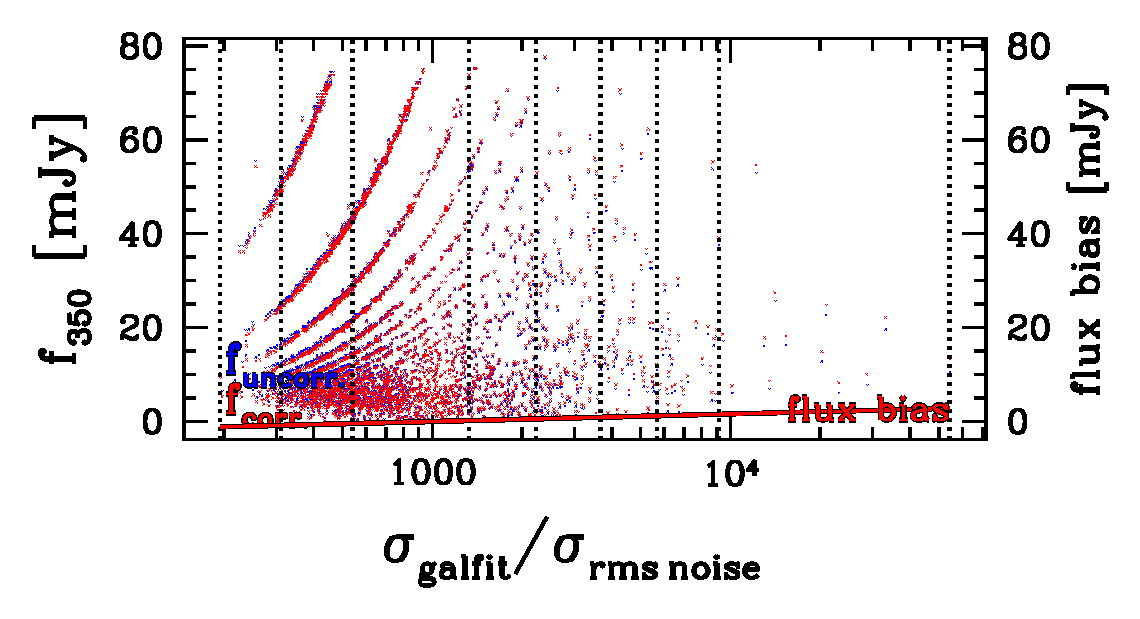
\includegraphics[width=0.65\textwidth]{galsim_350_fbias_1}
	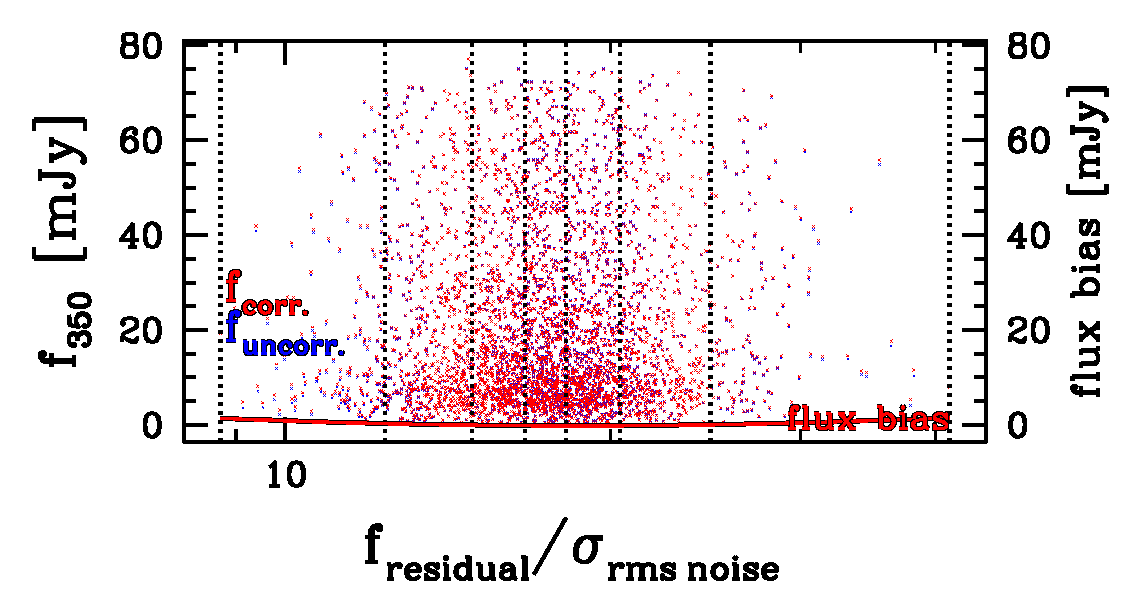
\includegraphics[width=0.65\textwidth]{galsim_350_fbias_2}
	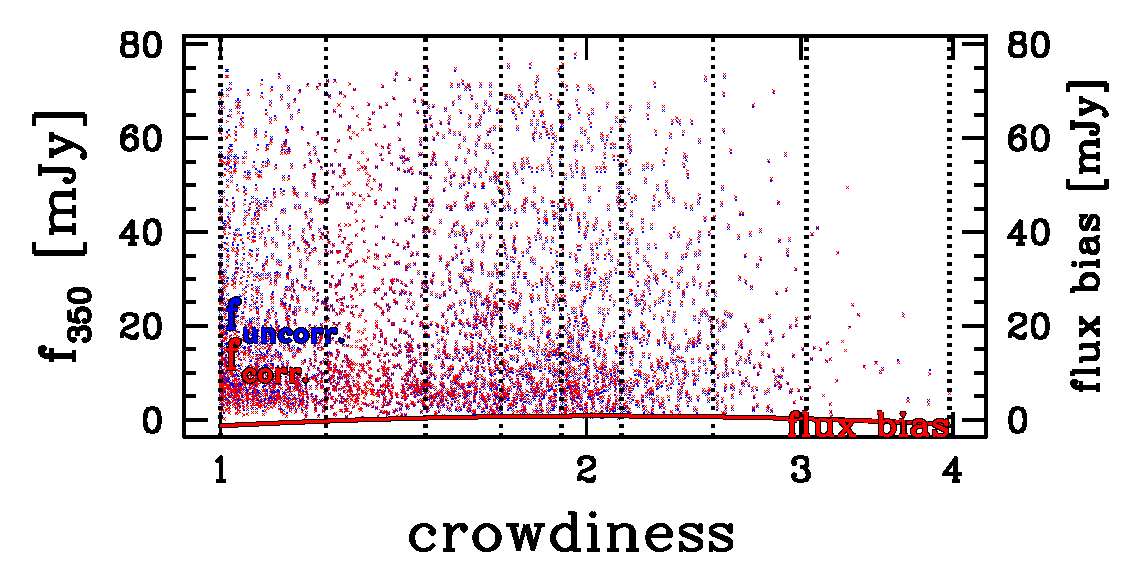
\includegraphics[width=0.65\textwidth]{galsim_350_fbias_3}
\end{figure}

\begin{figure}[H]
	\caption{
		\textcolor{red}{(TODO: Band 350 flux uncertainty correction plots:)}
	}
	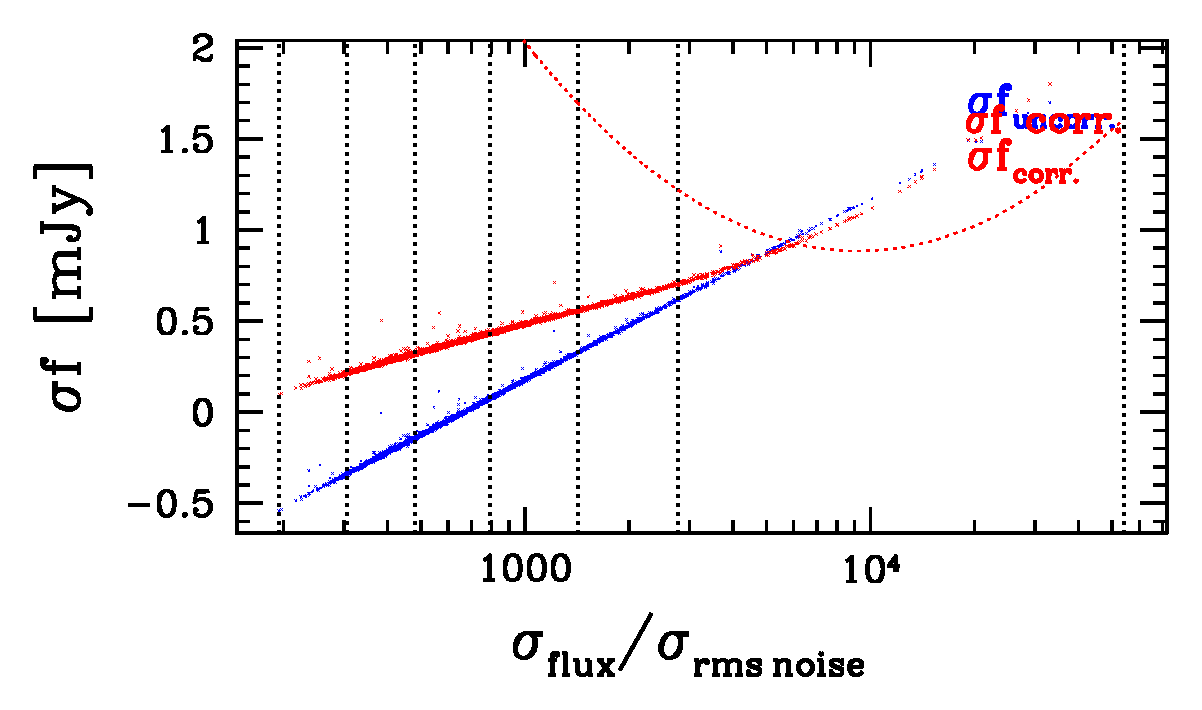
\includegraphics[width=0.65\textwidth]{galsim_350_dfcorr_1}
	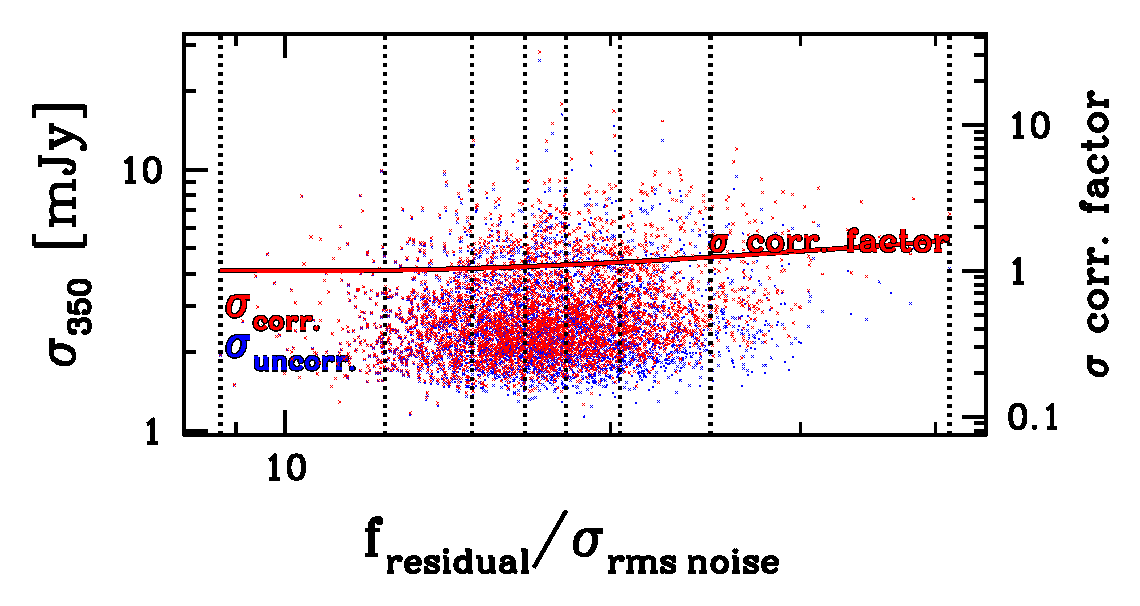
\includegraphics[width=0.65\textwidth]{galsim_350_dfcorr_2}
	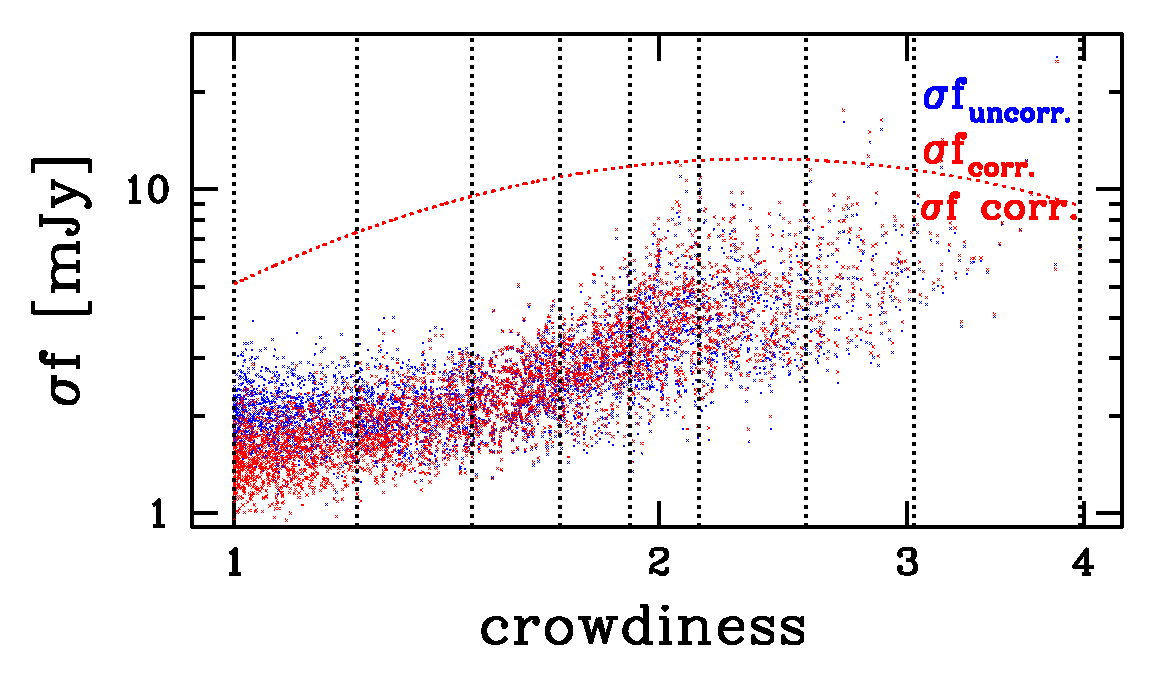
\includegraphics[width=0.65\textwidth]{galsim_350_dfcorr_3}
\end{figure}

%*************************************************************************************
\section{Band 500}

\subsection{SED fitting before band 500}
\label{Band500_Galsed}

Firstly, we use the Type\_AGN and Type\_SED determined in \ref{Band350_Galsed}:

\indent\hspace{15pt}$\bullet$ 
Type\_AGN: Numbers TODO. 
\\
\indent\hspace{15pt}$\bullet$ 
Type\_SED: Numbers TODO. 
\\
\indent\hspace{15pt}$\circ$ 
\textcolor{blue}{Note: \textcolor{blue}{do not forget} to append zeros for additional sources found in the residual image of 350.}
\\

Then we determine Type\_FIR with the latest 350 measurements:

\indent\hspace{15pt}$\bullet$ 
Type\_FIR: $\sqrt{SNR_{100}^2+SNR_{160}^2+SNR_{250}^2+SNR_{350}^2} \ge 5$: 1092 out of 3361 sources will be fit with only FIR data points. 
\\

\subsection{SED prediction for band 500}
\label{Band500_Galpre}

\begin{lstlisting}[language=bash]
cd Galsed_BeforeBand500_Pass2/do_Type_FIT
gedit do_Type_FIT.sm
define band 500
define fcut$band 1.02
define fmax$band 3.0
set catalog = {"../RadioOwenMIPS24_priors_v6_20151221_BeforeBand500.txt"}
set sedpredict = {"../ResLMTfluxes_priors_v6_20151221_BeforeBand500.txt"}
macro read do_Type_FIT.sm go
Total source number: 3361
Fitting source number: 386
Subtract source number: 2975
\end{lstlisting}

\begin{figure}[H]
	\caption{Number of sources kept for fitting per PSF beam area ($\rho_{fit}$) as a function of different $f_{cut}$ at band 500.}
	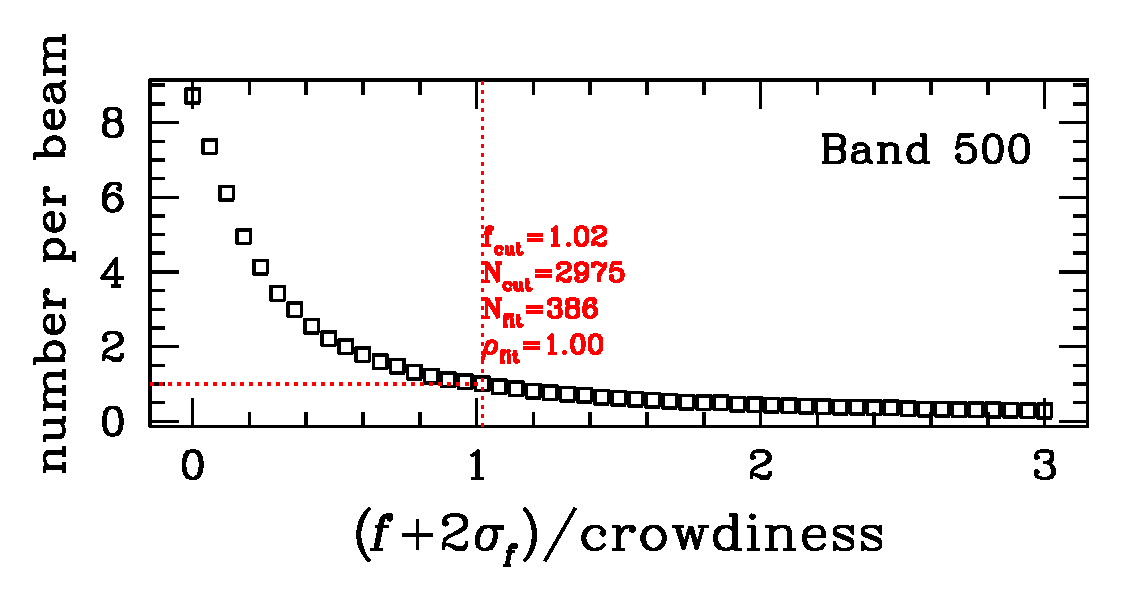
\includegraphics[width=0.85\textwidth]{plot_cutting_flux_500_with_crow}
\end{figure}

\subsection{Faint flux subtraction at band 500}
\label{Band500_Galsub}

We use the SED flux of the flagged faint sources to construct a PSF-modeled image, then subtract it from the original observed image. 

\begin{lstlisting}[language=bash]
./do_Galsub 500 201512 \
-catalog RadioOwenMIPS24_priors_v6_20151221_BeforeBand500.txt \
-fitsname spire500_ima_7p2_v0_100615.fits \
-sedpredict SED_predictions_500_201512.txt
\end{lstlisting}

\begin{figure}[H]
	\caption{Faint-source subtraction step at band 500. From left to right: original image, faint-source model image, and faint-source-subtracted image.}
%	\includegraphics[width=0.9\textwidth]{galfit_500_FIT_goodsn_500_Map_201512_Galsub}
%    TODO
\end{figure}

Using the faint-sources-subtracted image, we perform prior source fitting photometry in the next step. 

\indent\hspace{15pt}$\circ$ 
\textcolor{blue}{Note: Remember to set Xback=0 and fbias=0 while doing the faint-source subtraction.}
\\

\subsection{Galfit photometry at band 500}
\label{Band500_Galfit}

\begin{lstlisting}[language=bash]
./do_Galfit 500 201512 \
-catalog RadioOwenMIPS24_priors_v6_20151221_BeforeBand500.txt \
-fitsname spire500_ima_7p2_v0_100615_subfaintDL.fits \
-sedpredict SED_predictions_500_201512.txt
# then run scripts in parallel 
cd boxgalfit; do_GalfitRunqsub
cd ..
# then run postparallel process
./do_Galfit 500 201512 \
-catalog RadioOwenMIPS24_priors_v6_20151221_BeforeBand500.txt \
-fitsname spire500_ima_7p2_v0_100615_subfaintDL.fits \
-sedpredict SED_predictions_500_201512.txt \
-postparallel
\end{lstlisting}

\subsection{Residual image at band 500}
\label{Band500_Galres}

\begin{lstlisting}[language=bash]
cd run_sextractor_500/
idl -e 'do_SExtract_Mask, \
FitsFile="FIT_goodsn_500_Map_201512.fits", \
RmsFile="spire500_rms_7p2_v0_100615.fits"'
vim default.sex # set sigma thresholds
sex SExtractor_Signal.fits
# then write additional residual source catalog
# with supermongo code do_sextract_result.sm
gedit do_sextract_result.sm
...
define band 500
set catalog = {"RadioOwenMIPS24_priors_v6_20151221_BeforeBand500.txt"}
set rmsfits24 = {"n_mips_1_s1_v0_37_rms_ED.fits"}
set catalogadd = {"Residual_priors_v6_Band500.txt"}
...
print $(catalogadd) '%-9.0f %12.7f %12.7f %9g\n' \
{_id _ra _de zp_X f24 df24 f16 df16 f100 df100 \
f160 df160 f250 df250 f350 df350 radio eradio \
_fch1 _dfch1 _fch2 _dfch2 _fch3 _dfch3 _fch4 _dfch4 \
KtotX MassX distX spezX zq source distz idz goodArea}
...
macro read do_sextract_result.sm go
\end{lstlisting}

\textcolor{red}{(TODO: Put Residual Images Here!)}

Then run a second pass \ref{Band500_Galfit}: 

\begin{lstlisting}[language=bash]
./do_Galfit 500 201512 \
-catalog RadioOwenMIPS24_priors_v6_20151221_BeforeBand500.txt \
-catalog-add Residual_priors_v6_Band500.txt \ `\textcolor{blue}{\# ${new!}$}`
-fitsname spire500_ima_7p2_v0_100615_subfaintDL.fits \
-sedpredict SED_predictions_500_201512.txt
# then run scripts in parallel 
cd boxgalfit; do_GalfitRunqsub
cd ..
# then run postparallel process
./do_Galfit 500 201512 \
-catalog RadioOwenMIPS24_priors_v6_20151221_BeforeBand500.txt \
-catalog-add Residual_priors_v6_Band500.txt \ `\textcolor{blue}{\# ${new!}$}`
-fitsname spire500_ima_7p2_v0_100615_subfaintDL.fits \
-sedpredict SED_predictions_500_201512.txt \
-postparallel
\end{lstlisting}

\subsection{Monte-Carlo simulation at band 500}
\label{Band500_Galsim}

\subsection{Flux bias and flux uncertainty correction}
\label{Band500_dfcorr}

\begin{lstlisting}[language=bash]
gedit run_simu_stats_v6.sm
sm
macro read run_simu_stats_v6.sm run_simu_stats_v6 500
\end{lstlisting}

\begin{figure}[H]
	\caption{
		\textcolor{red}{(TODO: Band 500 flux bias correction plots:)}
	}
	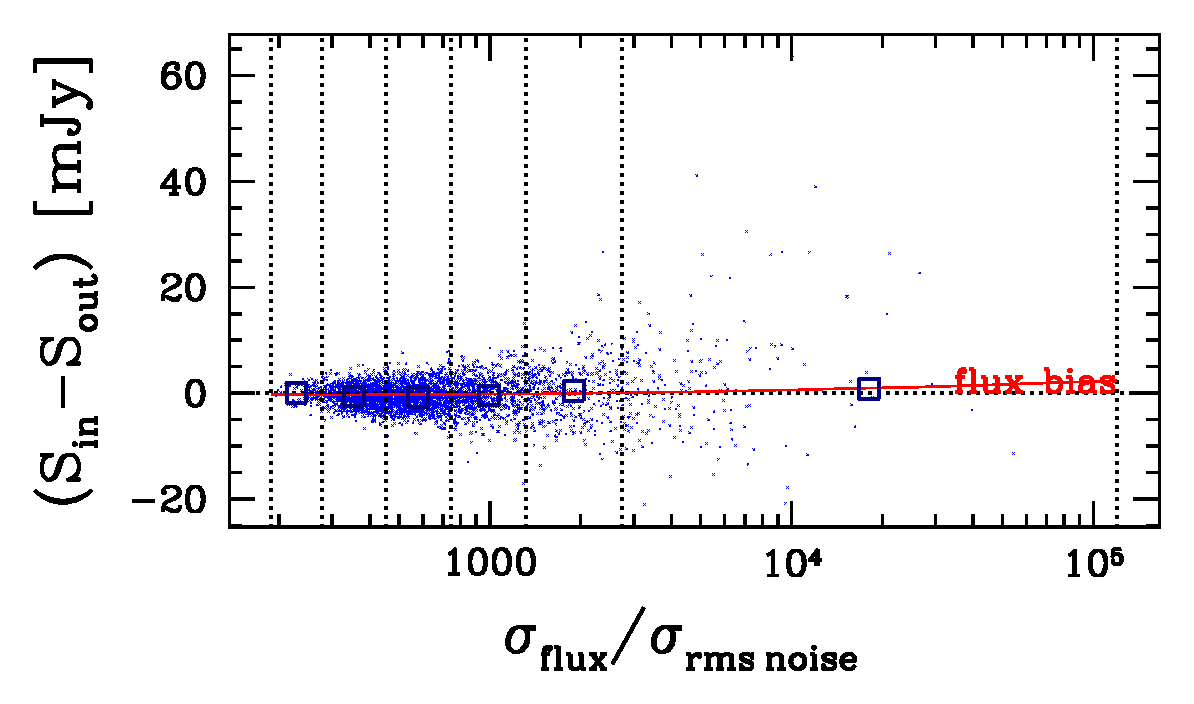
\includegraphics[width=0.65\textwidth]{galsim_500_fbias_1}
	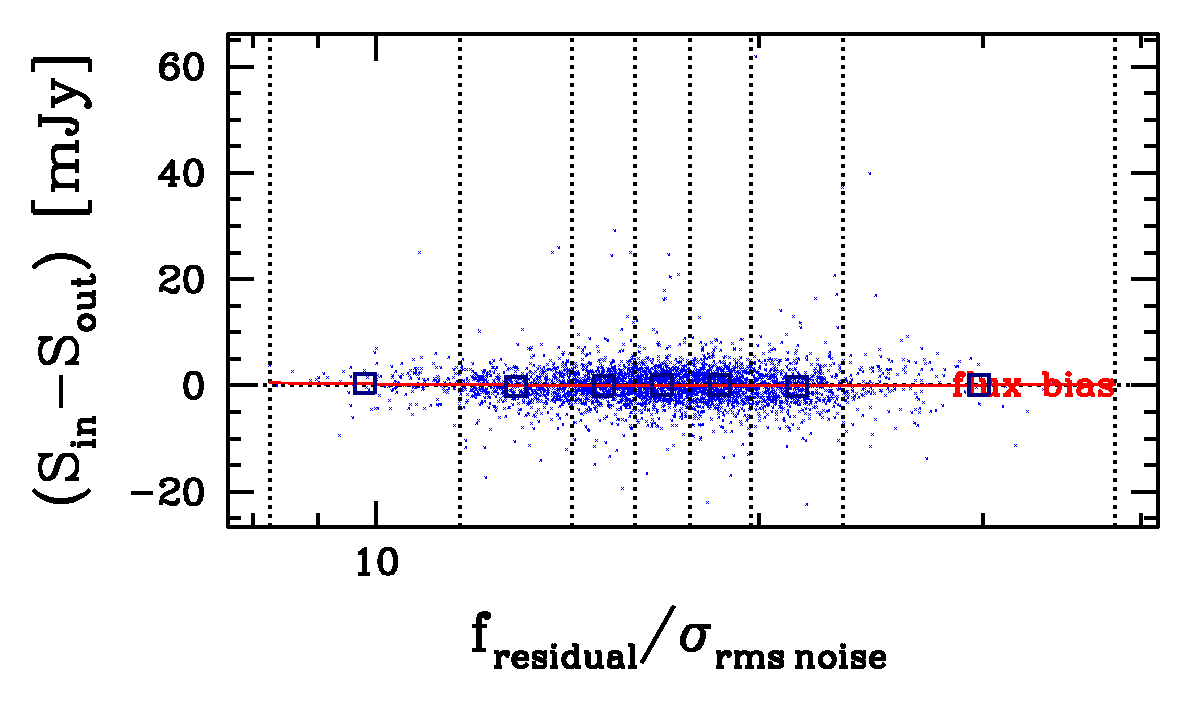
\includegraphics[width=0.65\textwidth]{galsim_500_fbias_2}
	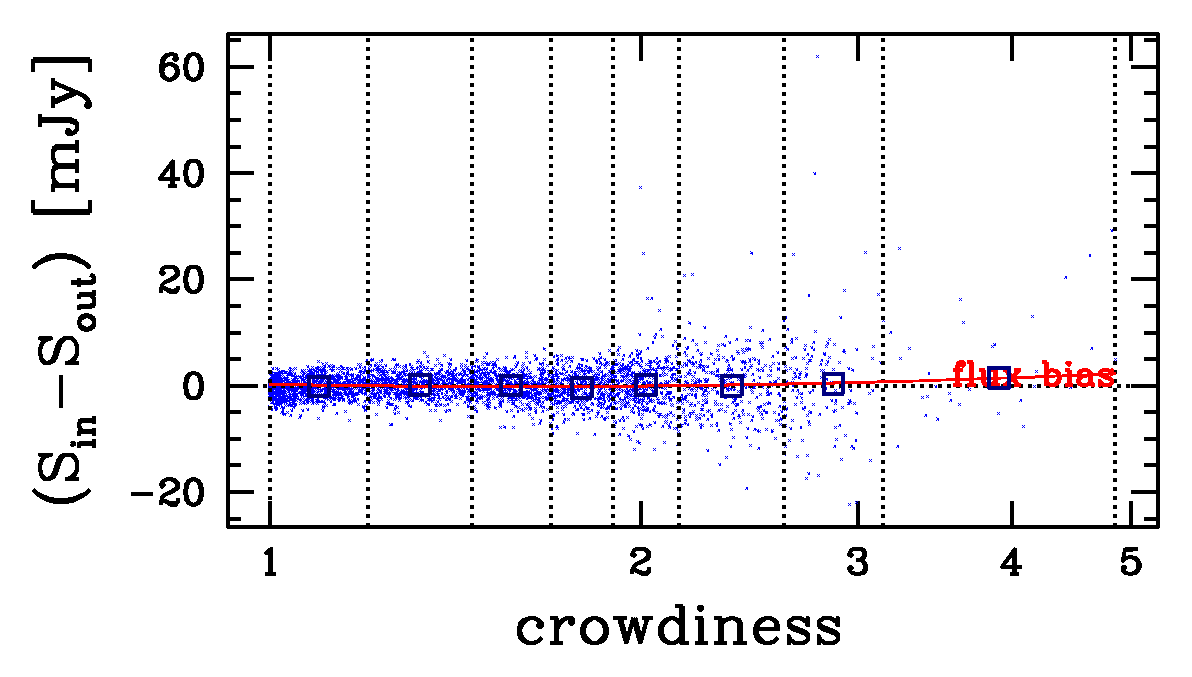
\includegraphics[width=0.65\textwidth]{galsim_500_fbias_3}
\end{figure}

\begin{figure}[H]
	\caption{
		\textcolor{red}{(TODO: Band 500 flux uncertainty correction plots:)}
	}
	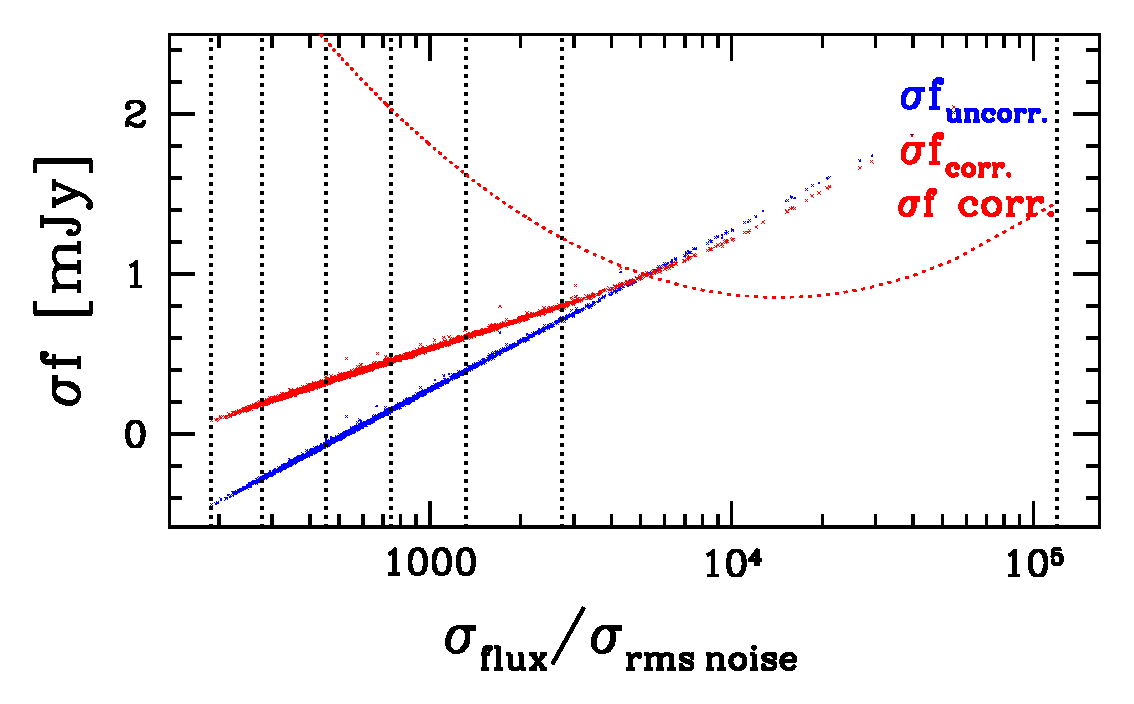
\includegraphics[width=0.65\textwidth]{galsim_500_dfcorr_1}
	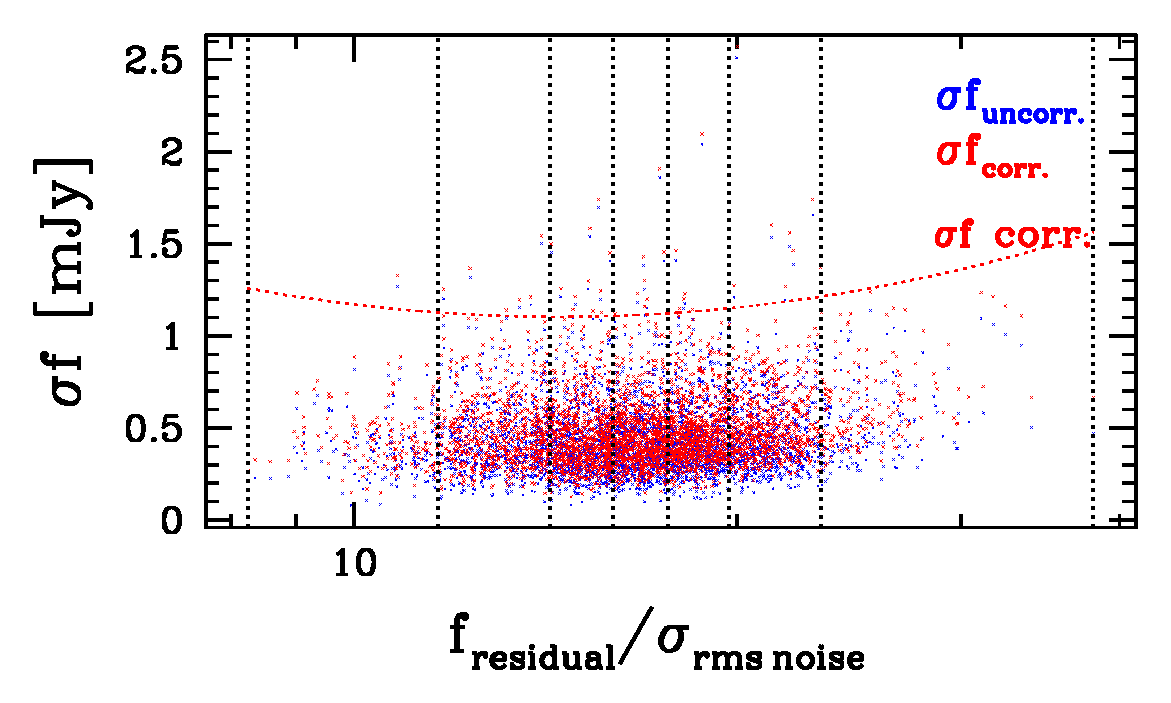
\includegraphics[width=0.65\textwidth]{galsim_500_dfcorr_2}
	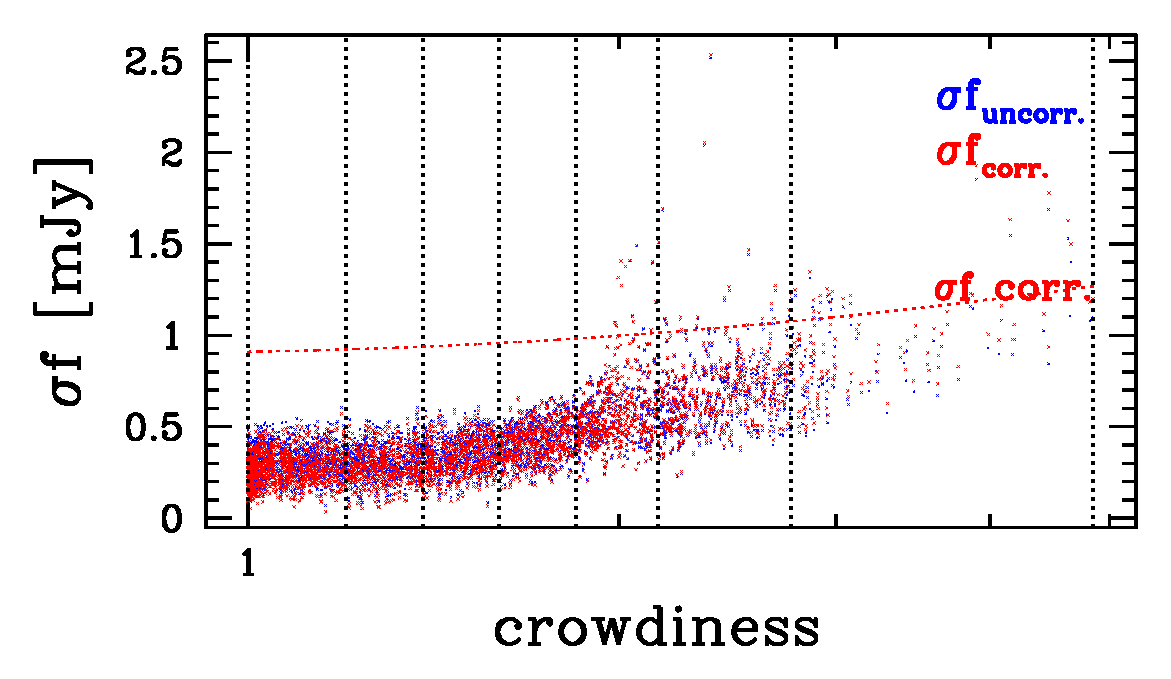
\includegraphics[width=0.65\textwidth]{galsim_500_dfcorr_3}
\end{figure}

%*************************************************************************************
\section{Band 1160}

\subsection{SED fitting before band 1160}
\label{Band1160_Galsed}

Firstly, we use the Type\_AGN and Type\_SED determined in \ref{Band500_Galsed}:

\indent\hspace{15pt}$\bullet$ 
Type\_AGN: Numbers TODO. 
\\
\indent\hspace{15pt}$\bullet$ 
Type\_SED: Numbers TODO. 
\\
\indent\hspace{15pt}$\circ$ 
\textcolor{blue}{Note: \textcolor{blue}{do not forget} to append zeros for additional sources found in the residual image of 500.}
\\

Then we determine Type\_FIR with the latest 500 measurements:

\indent\hspace{15pt}$\bullet$ 
Type\_FIR: $\sqrt{SNR_{100}^2+SNR_{160}^2+SNR_{250}^2+SNR_{350}^2+SNR_{500}^2} \ge 5$: 1114 out of 3386 sources will be fit with only FIR data points. 
\\

\subsection{SED prediction for band 1160}
\label{Band1160_Galpre}

\begin{lstlisting}[language=bash]
cd Galsed_BeforeBand1160_Pass2/do_Type_FIT
gedit do_Type_FIT.sm
define band 1160
define fcut$band 0.205
define fmax$band 0.75
set catalog = {"../RadioOwenMIPS24_priors_v6_20151221_BeforeBand1160.txt"}
set sedpredict = {"../ResLMTfluxes_priors_v6_20151221_BeforeBand1160.txt"}
macro read do_Type_FIT.sm go
Total source number: 3386
Fitting source number: 651
Subtract source number: 2735
\end{lstlisting}

\begin{figure}[H]
	\caption{Number of sources kept for fitting per PSF beam area ($\rho_{fit}$) as a function of different $f_{cut}$ at band 1160.}
	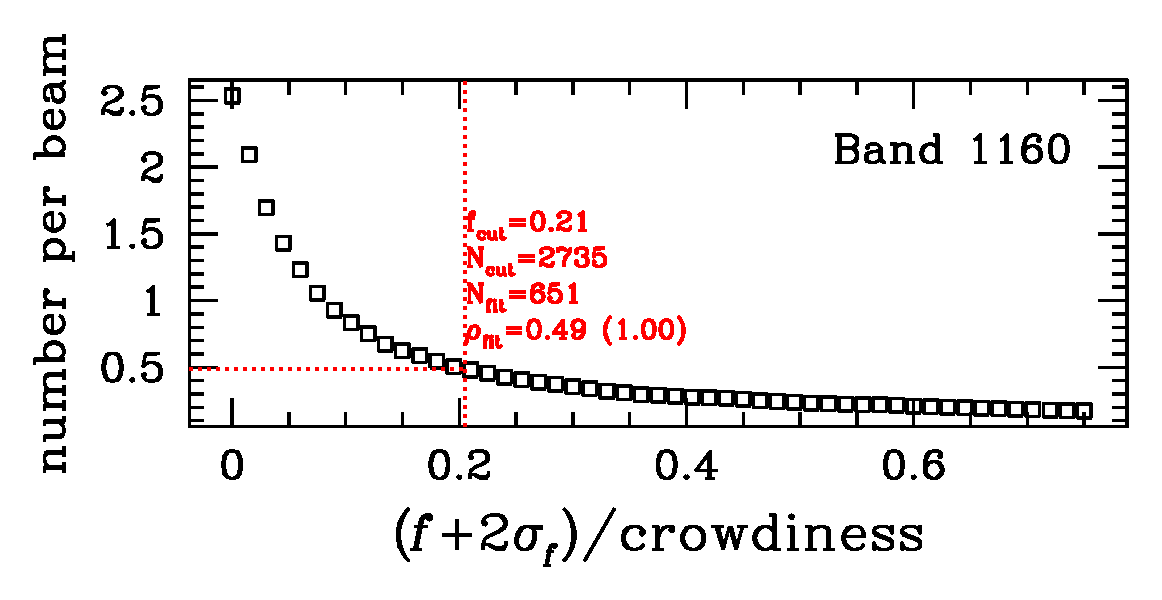
\includegraphics[width=0.85\textwidth]{plot_cutting_flux_1160_with_crow}
\end{figure}

\subsection{Faint flux subtraction at band 1160}
\label{Band1160_Galsub}

We use the SED flux of the flagged faint sources to construct a PSF-modeled image, then subtract it from the original observed image. 

\begin{lstlisting}[language=bash]
./do_Galsub 1160 201512 \
-catalog RadioOwenMIPS24_priors_v6_20151221_BeforeBand1160.txt \
-fitsname combined_maw0_4_azw0_5_sig_astro.fits \
-sedpredict SED_predictions_1160_201512.txt
\end{lstlisting}

\begin{figure}[H]
	\caption{Faint-source subtraction step at band 1160. From left to right: original image, faint-source model image, and faint-source-subtracted image.}
%	\includegraphics[width=0.9\textwidth]{galfit_1160_FIT_goodsn_1160_Map_201512_Galsub}
%    TODO
\end{figure}

Using the faint-sources-subtracted image, we perform prior source fitting photometry in the next step. 

\indent\hspace{15pt}$\circ$ 
\textcolor{blue}{Note: Remember to set Xback=0 and fbias=0 while doing the faint-source subtraction.}
\\

\subsection{Galfit photometry at band 1160}
\label{Band1160_Galfit}

\begin{lstlisting}[language=bash]
./do_Galfit 1160 201512 \
-catalog RadioOwenMIPS24_priors_v6_20151221_BeforeBand1160.txt \
-fitsname combined_maw0_4_azw0_5_sig_subfaintDL.fits \
-sedpredict SED_predictions_1160_201512.txt
# then run scripts in parallel 
cd boxgalfit; do_GalfitRunqsub`\textcolor{red}{255}`
cd ..
# then run postparallel process
./do_Galfit 1160 201512 \
-catalog RadioOwenMIPS24_priors_v6_20151221_BeforeBand1160.txt \
-fitsname combined_maw0_4_azw0_5_sig_subfaintDL.fits \
-sedpredict SED_predictions_1160_201512.txt \
-postparallel
\end{lstlisting}

\subsection{Residual image at band 1160}
\label{Band1160_Galres}

\begin{lstlisting}[language=bash]
cd run_sextractor_1160/
idl -e 'do_SExtract_Mask, \
FitsFile="FIT_goodsn_1160_Map_201512.fits", \
RmsFile="combined_maw0_4_azw0_5_rms.fits"'
vim default.sex # set sigma thresholds
sex SExtractor_Signal.fits
# then write additional residual source catalog
# with supermongo code do_sextract_result.sm
gedit do_sextract_result.sm
...
define band 1160
set catalog = {"RadioOwenMIPS24_priors_v6_20151221_BeforeBand1160.txt"}
set rmsfits24 = {"n_mips_1_s1_v0_37_rms_ED.fits"}
set catalogadd = {"Residual_priors_v6_Band1160.txt"}
...
print $(catalogadd) '%-9.0f %12.7f %12.7f %9g\n' \
{_id _ra _de zp_X f24 df24 f16 df16 f100 df100 f160 \
df160 f250 df250 f350 df350 f500 df500 radio eradio \
_fch1 _dfch1 _fch2 _dfch2 _fch3 _dfch3 _fch4 _dfch4 \
KtotX MassX distX spezX zq source distz idz goodArea}
...
macro read do_sextract_result.sm go
\end{lstlisting}

\textcolor{red}{(TODO: Put Residual Images Here!)}

Then run a second pass \ref{Band1160_Galfit}: 

\begin{lstlisting}[language=bash]
./do_Galfit 1160 201512 \
-catalog RadioOwenMIPS24_priors_v6_20151221_BeforeBand1160.txt \
-catalog-add Residual_priors_v6_Band1160.txt \ `\textcolor{blue}{\# ${new!}$}`
-fitsname combined_maw0_4_azw0_5_sig_subfaintDL.fits \
-sedpredict SED_predictions_1160_201512.txt
# then run scripts in parallel 
cd boxgalfit; do_GalfitRunqsub`\textcolor{red}{255}`
cd ..
# then run postparallel process
./do_Galfit 1160 201512 \
-catalog RadioOwenMIPS24_priors_v6_20151221_BeforeBand1160.txt \
-catalog-add Residual_priors_v6_Band1160.txt \ `\textcolor{blue}{\# ${new!}$}`
-fitsname combined_maw0_4_azw0_5_sig_subfaintDL.fits \
-sedpredict SED_predictions_1160_201512.txt \
-postparallel
\end{lstlisting}

\subsection{Monte-Carlo simulation at band 1160}
\label{Band1160_Galsim}

\subsection{Flux bias and flux uncertainty correction}
\label{Band1160_dfcorr}

\begin{lstlisting}[language=bash]
gedit run_simu_stats_v6.sm
sm
macro read run_simu_stats_v6.sm run_simu_stats_v6 1160
\end{lstlisting}

%\begin{figure}[H]
%	\caption{
%		\textcolor{red}{(TODO: Band 1160 flux bias correction plots:)}
%	}
%	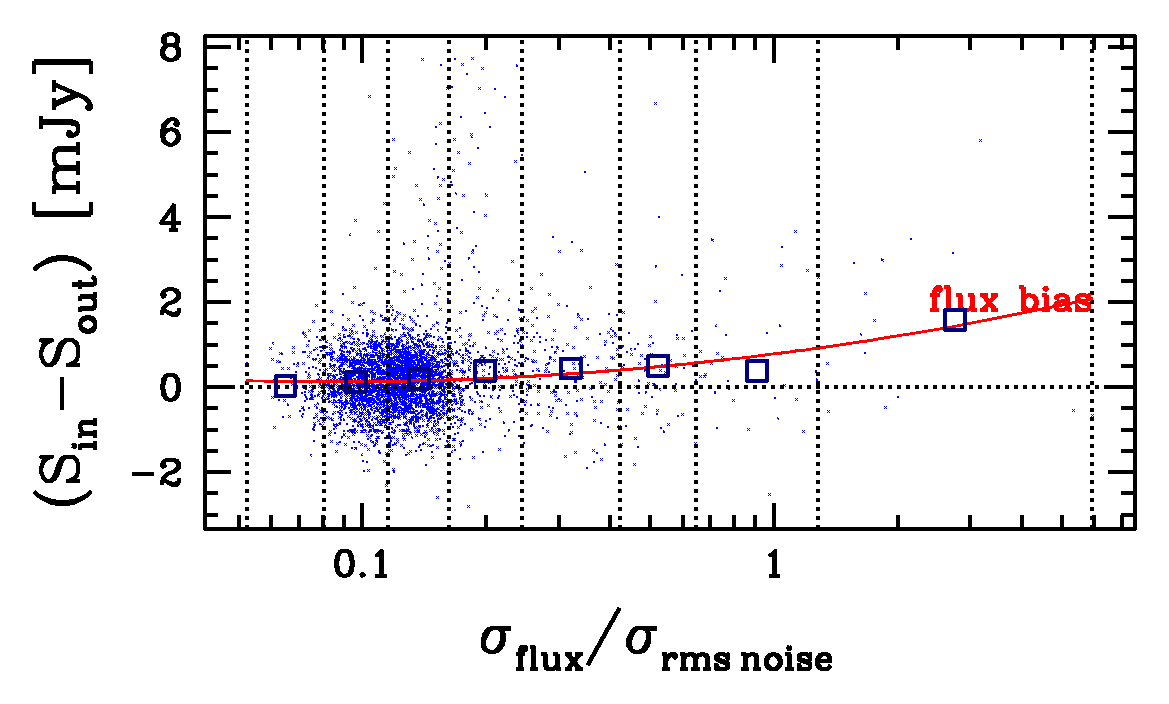
\includegraphics[width=0.65\textwidth]{galsim_1160_fbias_1}
%	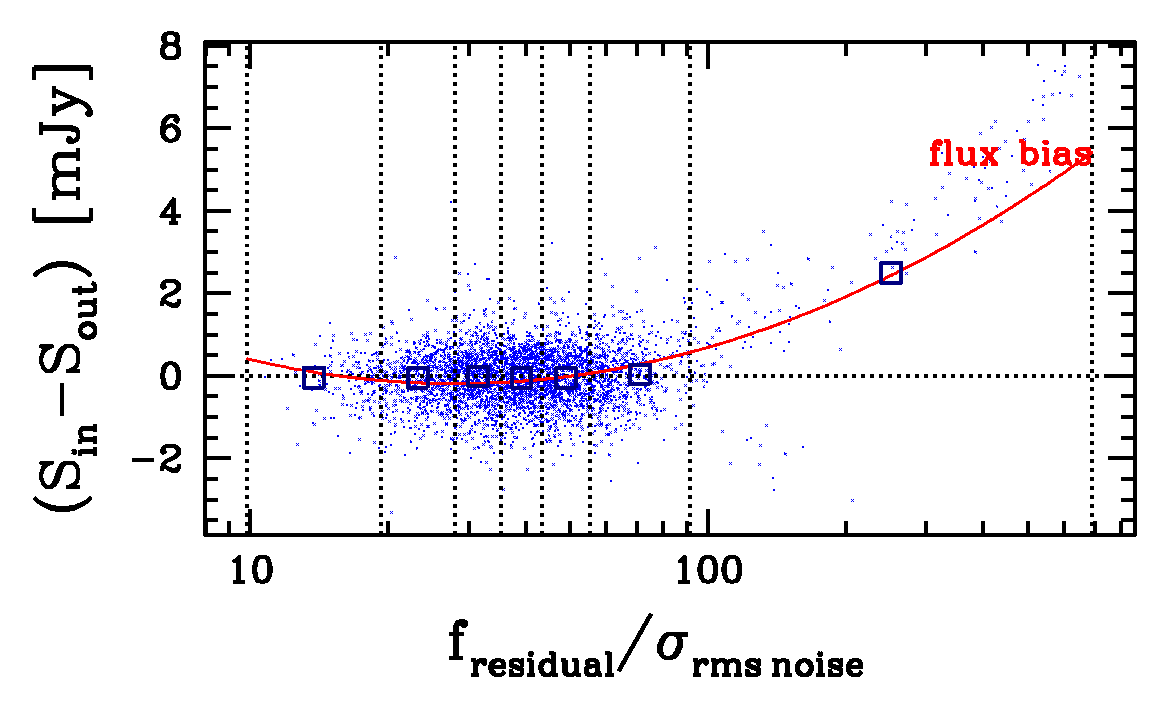
\includegraphics[width=0.65\textwidth]{galsim_1160_fbias_2}
%	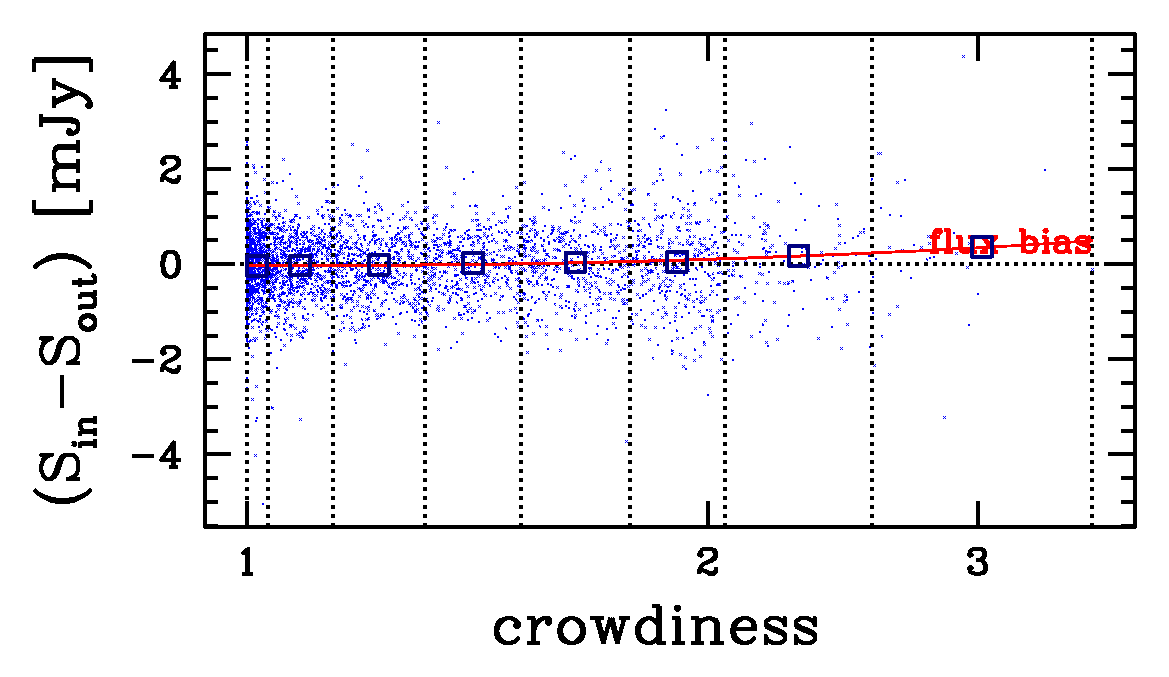
\includegraphics[width=0.65\textwidth]{galsim_1160_fbias_3}
%\end{figure}
%
%\begin{figure}[H]
%	\caption{
%		\textcolor{red}{(TODO: Band 1160 flux uncertainty correction plots:)}
%	}
%	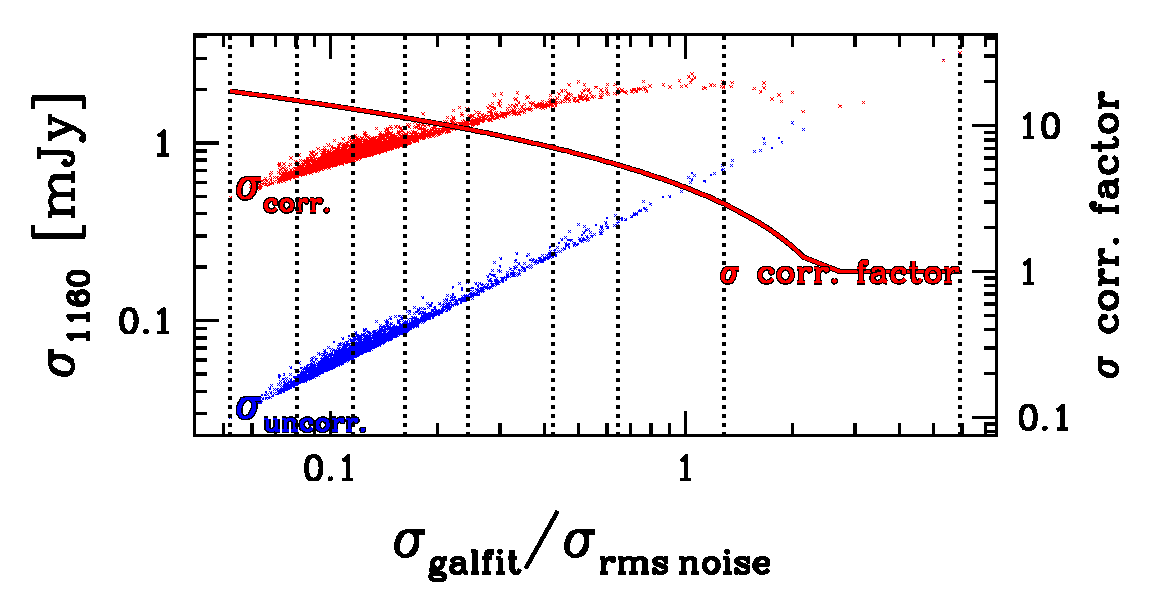
\includegraphics[width=0.65\textwidth]{galsim_1160_dfcorr_1}
%	\includegraphics[width=0.65\textwidth]{galsim_1160_dfcorr_2}
%	\includegraphics[width=0.65\textwidth]{galsim_1160_dfcorr_3}
%\end{figure}

%*************************************************************************************

\clearpage

%*************************************************************************************
\appendix

\section{Setup softwares in planer}
\label{Appendix_Software_Dependencies}

\begin{lstlisting}[language=bash]
IRAF
supermongo
galfit
sextractor
ds9
XPA # http://ds9.si.edu/site/XPA.html
wcstools # http://tdc-www.harvard.edu/software/wcstools/wcstools-3.9.2.tar.gz
others # 
\end{lstlisting}

\section{Setup supermongo in planer}
\label{Appendix_Supermongo}

Here are the code for configuring, compiling and installing supermongo: 

\begin{lstlisting}[language=bash]
cd /dsm/upgal/data/dliu/Software/sm2_4_30/
./set_opts
We can help you configure things for which the defaults are usually OK
Do you want to do so? [n|y|list] y
Choose data type for vectors, "float" or "double"? [float] double
Choose length of longest macro [10000] 50000
Choose length for string-valued-vectors' elements [40] 80
Top level path to install things? [/usr/local] /dsm/upgal/data/dliu/supermongo
vim src/options.h
:d7
:wq
make
make install
cd
cd /home/dliu/.local/lib/sm/macro
rsyncdir /usr/local/lib/sm/macro \
dliu@hubble.extra.cea.fr:/dsm/upgal/data/dliu/supermongo/lib/sm/macro "*.sm"
It should be OK now!
echo PATH=/home/dliu/.local/bin:$PATH
type sm
# Note:
# additionally, if sm does not work, 
# try to modify "/home/dliu/.local/lib/sm/.sm"
\end{lstlisting}

\end{document}